\documentclass[a4j]{ltjreport}
%\documentclass[a4j]{ltjsreport} <= 2022Ver!
% "'h' float specifier changed to 'ht'"の警告はあまり気にしなくて良いらしい?
%LaTeX有識者に改良求む...
%あとMarkdown形式への移行の計画があるようですが綿貫が途中で力尽きた場合は
%次の担当者にお任せしたいです......

\topmargin -0.4in
\oddsidemargin -0.3in
\textheight 9in
\textwidth 7in
\columnsep 0.4in

\usepackage[match,deluxe,bold]{luatexja-preset}
%\usepackage[match,deluxe,bold,noto-otf]{luatexja-preset} <= 2022Ver
%フォントの問題でnoto-otfは使わず.
\usepackage{amsmath, amssymb}
\usepackage{here}
\usepackage{graphicx}
\usepackage{overpic}
\usepackage{ascmac}
\usepackage{color}
\usepackage{url}
\usepackage{fancyvrb}
\usepackage{longtable}
\usepackage{listings}
\usepackage{jvlisting}
\usepackage{multirow}
\usepackage{comment}
\usepackage[hidelinks,unicode]{hyperref}

\lstset{
numbers=left,
frame=single,
basicstyle={\ttfamily},
}

\setcounter{tocdepth}{2}

\newcommand{\cn}[1]{\multirow{2}{*}{#1}}

\title{\textbf{地球惑星物理学科 計算機演習}\\
$\sim$ Unix2 $\sim$}
\author{綿貫 元起\thanks{固体地球科学講座 安藤研究室 修士1年}\footnote{\copyright 本資料は歴代の地球惑星物理学科の先輩方によって作成されたものを再構成・改訂して作成しています}}

\date{令和5年4月10日}

\begin{document}
    \maketitle

    \chapter*{はじめに}
    計算機演習も3回目となりました。
    基本的な部分は前回習ったと思いますので、
    今回は少し発展的ですが知っておくと非常に便利な事柄について学んでいきます。
    また、慣れないことが続き消化不良に陥っている人も居るかと思いますので、
    コマンドラインでのファイル操作の復習も兼ねて行います。

    Unix端末は、最初はとっつきにくい部分もありますが、
    使いこなせるようになれば、他の汎用OS以上の機能や
    カスタマイズ性を実現することができます。そのためにシステムの
    理解は不可欠であり、講義の後半ではそのための基礎的な知識を
    説明します。

    本テキストはPythonの導入にともなって削除された中盤のTA担当授業Shell 1\footnote{2007 年度シェルその2
    (吉武さん製作)およびシェルその3(落さん製作)を参考に作成された2009 年度テキスト(竹尾さん製作)
    を参考に作成された2010 年度テキスト(若松さん製作)を参考にして作成された2011 年度テキスト
    (平林さん製作)を参考にした2013 年度テキスト(末松さん制作)を参考にした2014 年テキスト(菅野さん作成)
    を参考にした2016 年テキスト(松岸さん作成) を参考にした2018 年テキスト(柳町さん作成)
    を参考にした2019 年テキスト(池端さん作成) を参考にした2020 年テキスト(加藤さん作成) 
    を参考した2021年テキスト(細谷さん作成)にしています。}, 
    Shell 2\footnote{2010 年の松井さん、2012 年の小池さん、2013 年の西川さん、2017 年の小澤さん、
    2018 年の灘本さんが作成してこられた資料の内容に、2020 年と2021 年に大竹と茂木が加筆修正し、
    課題を一部変更しました。}の内容を元のUNIX 2\footnote{2008 年に三木順哉さんによって作成されたもの
    を元に作成}のテキストにマージし編集して作られた
    2022年度テキスト\footnote{森さん作成}をさらに改訂して作成されています\footnote{改訂時さらに2019年度UNIX1のテキストの一部もマージしました。}。
    極めて内容過多かつ先取りをしているため、今日すぐにすべてをマスターする必要はありません。
    今日は\textbf{2章まで}をしっかりと身につけていただくことを目標にしています。
    3章以降はこれから様々な課題をこなす中でゆっくりと咀嚼していただければと思います。
    また、分からない内容があったら気軽にTAに聞いてください。
    %来年度以降の担当者へ:以降もshellが復活しなかった場合、喋るのは3.1節くらいまでで多分十分です.
    %第4章は好みに合わせて.

    \section*{配付資料の説明}
    今日使うファイルはdover上の \verb+/home0/watanuki2023/Unix2_Haifu/+ にある
    exerciseディレクトリとshell2ディレクトリに含まれています。
    とりあえず\verb+Unix2_Haifu+を丸々自分のディレクトリにコピーしましょう。
    見つからない場合はsakura上の \verb+/home0/mori2021/TA2021/exercise/+ および
    dover 上の \verb+/home0/ohtake2022/shell2/+ を探してみてください\footnote{どうしても見つからない場合はSlackで配布するなどして対処します。}
    \footnote{この資料において、sshコマンドとscpコマンドは559室で実施する場合を想定しています。
    もしリモートで、かつ\textasciitilde/.ssh/configを書いていない場合には、
    doverの部分をs2326**@dover.eps.s.u-tokyo.ac.jpに書き換えてください。}。
    \begin{lstlisting}[numbers=none]
    ~$ scp -r dover:/home0/watanuki2023/Unix2_Haifu/ .
    \end{lstlisting}

    コピーしたら、以下のコンテンツが揃っているか確認してください。

    \begin{itemize}
        \item words.txt, stations.txt, sample01.sh $\sim$ sample09.sh ::サンプルファイルです。テキストを読みながら適宜使ってください。(sample04.shとsample08.shを作るのは練習問題なので、ありません)。
        \item earthquake.txt, line.sh, students.txt :: これもテキストを読む際に使用します。
        \item shell2\_2021.pdf ::2021年版Shell 2テキストの電子版です。コピペしたいとかあれば使ってください。
        %\item (ディレクトリ) 2016\_02, 2017\_02, 2017\_11, 2018\_01, (ファイル) authors.txt ::提出してもらう課題に関するファイルです。最終章の課題に関する説明を読んでから使ってください。
    \end{itemize}


    \tableofcontents

    \chapter{これまでの復習}
    \section{基本的なコマンドとオプション}
    ターミナル上で次のようなコマンドを利用して、ファイル操作に慣れましょう。
    \begin{table}[htbp]
        \centering
        \caption{基本的なコマンド}
        \label{tab:command}
        \begin{tabular}{cccc}
            \hline
            \hline
            コマンド名   & 語源                     & 概要                       &  重要オプション \\
            \hline
            \texttt{cd}    &  Change Directory        & カレントディレクトリの移動 & - \\
            \texttt{pwd}   &  Print Working Directory & カレントディレクトリの表示 & \\
            \texttt{ls}    &  LiSt                    & ファイル一覧の表示         &	   -l -a -d -h -F \\
            \texttt{cp}    &  CoPy                    & ファイルの複製             &	      -R -f \\
            \texttt{mkdir} &  Make Directory          & ディレクトリの作成         &	      -p \\
            \texttt{mv}    &  MoVe                    & ファイルの移動 / リネーム  & \\
            \texttt{rm}    &  ReMove                  & ファイルの削除             &	      -r -f -i \\
            \texttt{rmdir} &  ReMove DIRectory        & ディレクトリの削除         &	      -p \\
            \hline
            \hline
        \end{tabular}
    \end{table}

    前回の講義でオプションについても習いました。例えば、ターミナルで
    \underline{\texttt{ls -R}}と
    入力してみましょう
    \footnote{ディレクトリ内容の再帰的表示が中々止まらない場合はcontrol+C等を試してみてください.}。
    どうなりましたか?これはどんなオプションでしょうか。
    \underline{\texttt{man ls}}として、確認してみましょう。また、一度に複数
    のオプションも使用できましたね。\underline{\texttt{ls -la}}と入力してみてください。
    これは\underline{\texttt{ls -a -l}} と同じ結果となるはずです。
    コマンドの機能を忘れてしまったときは\underline{\texttt{man <コマンド名>}}とするか、
    それでもわからなければGoogleなどで検索するとよいでしょう。
    \begin{verbatim}
    合計 108
    drwxr-xr-x  12 ueda student  4096  4月 10 14:24 ./
    drwxr-xr-x 305 root root    12288  3月 31 17:59 ../
    -rw-------   1 ueda ta         51  4月 10 14:24 .Xauthority
    -rw-r--r--   1 ueda ta       5837  3月 31 17:47 .Xresources
    -rw-r--r--   1 ueda ta        543  3月 31 17:47 .aliases
    drwx------   2 ueda ta       4096  4月  5 18:20 .anthy/
    -rw-------   1 ueda ta       1571  4月  5 18:49 .bash_history
    -rw-r--r--   1 ueda ta        416  3月 31 17:47 .bash_profile
    -rw-r--r--   1 ueda ta        973  3月 31 17:47 .bashrc
    drwx------   3 ueda ta       4096  4月  5 16:07 .dbus/
    -rw-r--r--   1 ueda ta       4120  3月 31 17:47 .emacs
    drwx------   3 ueda ta       4096  4月  5 17:49 .emacs.d/
    drwxr-xr-x   5 ueda ta       4096  3月 31 17:47 .fluxbox/
    drwx------   2 ueda ta       4096  4月 10 14:24 .gconf/
    drwxr-xr-x   3 ueda ta       4096  4月  5 16:07 .local/
    drwxr-xr-x   3 ueda ta       4096  4月  5 18:40 .texmf-var/
    drwx------   3 ueda ta       4096  3月 31 17:47 .uim.d/
    -rw-r--r--   1 ueda ta       5230  3月 31 17:47 .vimrc
    -rw-------   1 ueda ta        577  4月  5 18:47 .xdvirc
    \end{verbatim}

    ここに載せている以外にも様々な隠しファイル(ピリオドで始まるファイル)や
    前回までに作成したファイルが見えると思います。\verb+ls -l+の出力に
    関しては前回(UNIX その1)の講義で習いましたが、ちゃんと意味が理解できるでしょうか。

    一列目にある文字はパーミッションを表しています。パーミッションに関しては、
    「聞いたことはあるがどのようなものなのかよく分からない......」という方が
    多いと思うので、以下でちゃんと触れようと思います。

    また、隠しファイル(.bashrcなど)は主にユーザ毎の設定ファイルということでした。
    隠しファイルの設定に関しては、後ほどもう少し詳しく説明したいと思います。

    \subsection{練習}
    いくつかのコマンドとオプションを使って、遊んでみましょう。
    例えば、asanoに入り\underline{\texttt{sl}}コマンドを実行してみましょう。
    これは何のためのコマンドでしょうか?このコマンドは
    個人用PCにインストールすることもできるのでぜひ試してみてください。
    そして、\underline{\texttt{man sl}}としましょう。
    また、そこで見つけたオプションを試してみましょう。
    \underline{\texttt{cal -jy}}とかもやってみましょう。

    また\underline{\texttt{du}}は便利なコマンドの1つです\footnote{大きなデータを扱う際にお世話になるかもしれません.}。
    \underline{\texttt{du -sh}}として、
    それぞれのオプションの意味を\underline{\texttt{man du}}で確認してみてください。
    また、\underline{\texttt{du -sh *}}と入力してみましょう。

    (時間が余った人は \underline{\texttt{finger}}や\underline{\texttt{last}}, 
    \underline{\texttt{who}} なども調べてみると面白いかもしれません)

    また、ファイル操作に関するコマンドは非常に重要です。
    別の場所にあるディレクトリを自分のホームディレクトリにコピーするにはどうすればよいでしょうか?
    まだ「配布資料」を自分のホームディレクトリにコピーできていない方はここで試してみてください。
    
    なお、ファイル・ディレクトリの作成・削除、移動の仕方などが分からない人はTAの人に聞きながら練習してみてください。


%%%%%%%%%%%%%%%%%%%%%%%%%%%%%%%%%%%%%%%%%%%%%%%%%%%%%%%%%%%%%%%%%%
%この部分は2019年度計算機演習のUnix1から拝借.
%オリジナルのLaTeXコードは無かったのでpdfを参考にして改めて書いた
%(そのためオリジナルとは若干違う).


    \section{ユーザ・グループ・パーミッション}

    \subsection{スーパーユーザ}
    UNIX には スーパーユーザ (root) という特殊なユーザがいます。root ユーザはシステム管理をするため
    のユーザで、他のユーザのファイルを消したり、ユーザそのものを追加したり消去したり、アカウントを
    停止したり、他のユーザやシステム全体のプロセスを止めたり、とにかく何でもできるユーザです。559 で
    は admin210 という学生の管理者集団がボランティアで 559 のシステムを管理しており、admin210 のメン
    バーたちが root 権限を持っています。

    \subsection{ユーザとグループ}
    ユーザにはユーザ名と所属グループという情報があります。ユーザ名は説明するまでもなく、自分のユー
    ザ名です。所属グループは自分の所属するグループであって、ユーザは少くとも一つのグループに所属し、
    複数のグループに所属することもできます。ユーザの所属するグループのうち一つは特別なグループでプ
    ライマリグループと呼ばれ、ファイルなどを作成した時にそのファイルの所有グループとして使われます。

    グループへの所属登録自体は管理者 (root) が行います。また、ユーザ名やグループ名には数値で表され
    た識別子 (ID) が関連付けられています。id コマンドを使うことで自分や他のユーザの情報を見ることがで
    きます。

    \vspace*{1mm}
    \begin{lstlisting}[numbers=none]
        ~$ id
    \end{lstlisting}
    \vspace*{1mm}
    と打ってみてください。

    \vspace*{1mm}
    \begin{lstlisting}[numbers=none]
        ~$ uid=52132(s212632) gid=20000(student) groups=20000(student)...
    \end{lstlisting}
    \vspace*{1mm}
    のように出力されたと思います。

    これによって得られる表示のうち uid はユーザ ID とユーザ名、gid はプライマリグループ ID とプライ
    マリグループ名、groups は自分の所属する全グループ ID とグループ名です。

    このように、559 では学生ユーザはみな student というグループに所属しています。admin210 のメン
    バーになるとこの他 admin (gid=21000) というグループにも所属するようになります。TA や教員は
    ta (gid=20090) というグループに所属しています。また、

    \vspace*{1mm}
    \begin{lstlisting}[numbers=none]
        ~$ id username
    \end{lstlisting}
    \vspace*{1mm}
    でユーザusernameの情報を見ることができます。


    \subsection{ファイルの所有者}
    UNIXではそのファイルが誰のものかを

    \begin{enumerate}
        \item owner(所有者)
        \item group(所有グループ)
        \item other(他人)
    \end{enumerate}
    の 3 つに分けて区別しています。1. はそのファイルを所有する者、2. はそのファイルを
    所有するグループです。3. は所有者でなく 2. のグループにも属さないユーザを表わします。

    自分の所有するファイルでも owner を変更することはできませんが (root にはできます)、自分の所有す
    るファイルなら自分の所属するグループのいずれかへファイルのグループを変更できます。このときに利
    用するコマンドは chgrp です。

    \vspace*{1mm}
    \begin{lstlisting}[numbers=none]
        ~$ chgrp groupname filename
    \end{lstlisting}
    \vspace*{1mm}

    これでファイル filename の所有グループが groupname に変更されます。
    ディレクトリの中身も全て所有グループを変えたいのならば「-R」オプションをつけます。

    \vspace*{1mm}
    \begin{lstlisting}[numbers=none]
        ~$ chgrp -R groupname dirname
    \end{lstlisting}
    \vspace*{1mm}

    但し、自分の所属しないグループを所有グループにすることはできませんので 
    student グループにしか所属していない皆さんは chgrp コマンドを使うことはないでしょう。

    \subsection{パーミッション}
    ファイルやディレクトリに対するアクセス許可のことをパーミッションといいます。
    owner/group/otherに対して

    \begin{itemize}
        \item r:  読み取り許可
        \item w:  書き込み許可
        \item x:  実行許可
    \end{itemize}

    を与えることができ、また、複数組み合わせることもできます。これらの意味するところはファイルかディ
    レクトリかで異っており、次の表のようになります。

    \begin{table}[htb]
        \centering
          \begin{tabular}{|l|c|c|c|}  \hline
              & ファイル & ディレクトリ  \\ \hline 
            \textbf{r} & ファイルへの読み込み & ディレクトリ内のファイル一覧取得 \\ \hline
            \textbf{w} & ファイルへの書き込み & ディレクトリ内のファイル作成・削除  \\ \hline
            \textbf{x} & 実行 & ディレクトリ内へのアクセス \\ \hline
          \end{tabular}
    \end{table}

    ただし、ディレクトリ内へのアクセスとは、そのディレクトリをカレントディレクトリにする、そのディレクト
    リの下のファイルを参照する、ということです。また、ディレクトリに r が付与されていなくても x が付
    与されていれば、その中のファイルにアクセスすることができます(もちろん、ファイルそのものに適切
    なパーミッション設定がされていなければなりません)。

    パーミッションを確認するにはコマンド ls に -l (エル) オプションをつけて使います。

    \vspace*{1mm}
    \begin{lstlisting}[numbers=none]
        ~$ ls -l
    \end{lstlisting}
    \vspace*{1mm}

    これで出てくる

    \vspace*{1mm}
    \begin{lstlisting}[numbers=none]
        ~$ -rw-rw-r-- ...
    \end{lstlisting}
    \vspace*{1mm}

    のような表示がそのファイルに設定されているパーミッションになります。
    この 10 個のパートは以下のように解釈します。

    \begin{table}[htb]
        \centering
          \begin{tabular}{|l|l|}  \hline
              最初の1文字が& d ならディレクトリ、- ならファイル  \\ \hline 
            それ以降 & 3文字1セットで解釈\\
              & 最初の3文字: 持ち主\\
              & 次の3文字: グループ\\
              & 最後の3文字: 他人\\\hline
             & そのそれぞれの意味   \\
             & r: 読んで良い(read)\\
             & w: 書いて良い(write)\\
             & x: 実行して良い(excute)\\
             & -: (その場所に応じて)許可しない\\ \hline
          \end{tabular}
    \end{table}

    \pagebreak
    パーミッションはowner/group/otherごとに

    \begin{table}[htb]
        \centering
          \begin{tabular}{|l|c|c|c|c|}  \hline
            許可の種類& r & w & z & -(不許可) \\ \hline 
            表す数 & 4 & 2 & 1 & 0 \\ \hline
          \end{tabular}
    \end{table}
    
    の3数の和で表されることもあります (ディレクトリであるかどうかは評価されません)。
    例えば、-rw-rw-r--や -rwx---r-x はそれぞれ664および705と表現されます。
    この 3 数の和で表現する方法はビット演算 (2 進数演算) を利用してい
    ることから、「owner に r ビットが立っている」などの言い方をすることもあります。

    \subsection{chmod}
    ファイルやディレクトリのパーミッションを変更するには chmod コマンド(change mode)を用います。
    使い方については man コマンドで調べてみましょう。

    \subsection{umask}
    umask 値はファイルやディレクトリを新規作成するときのパーミッションをいくつにするかという設定
    です。この値はファイルなら 666 の補数、ディレクトリなら 777 の補数であらわされます。どういうこと
    かというと、umask=022 のとき新規作成されるファイルは (繰り下げを許さない) 8 進数の引き算で 666 -
    022 = 644 で 644 となり、umask=022 のとき新規作成されるディレクトリは (繰り下げを許さない) 8 進数
    の引き算で 777 - 022 = 755 で 755 となる、といった具合です。

    他のユーザに自分のファイルを見られたくないと思ったら umask 値を 044、他のユーザに自分のファイ
    ルを編集されたくないと思ったら umask 値を 022、見せたくもないし編集もさせたくないと思ったら 066、
    といった感じです。ちょっと複雑ですが、理解しておきましょう。

    この umask 値はデフォルトでシステム規定の値となっていますが、umask コマンドでその値を知ること
    ができます。また、umask コマンドに設定したい umask 値を引数で与えてやれば設定をかえることもでき
    ます。例えば、

    \vspace*{1mm}
    \begin{lstlisting}[numbers=none]
        ~$ umask
    \end{lstlisting}
    \vspace*{1mm}

    とすると現在のumask値が表示され、

    \vspace*{1mm}
    \begin{lstlisting}[numbers=none]
        ~$ umask 002
    \end{lstlisting}
    \vspace*{1mm}
    とするとumask値が002に設定されます。



%%%%%%%%%%%%%%%%%%%%%%%%%%%%%%%%%%%%%%%%%%%%%%%%%%%%%%%%%%%%%%%%%%

\pagebreak
    \section{リダイレクトとパイプ}
    さて次も前回習った話です。
    パイプはUNIXの哲学の根幹にあるという話でした。
    使えるようになっているでしょうか?
    \textbf{標準出力をファイルに書き出したり、ファイルの中身を標準入力として読み込んだりする際に使うのがリダイレクト}、
    \textbf{標準出力を別の操作の標準入力として送り込むのがパイプ}でした。
    それぞれについて、前回の講義で簡単な例を用いて学習したと思います。
    ここでは、\verb+head+と\verb+tail+というコマンドを使って、パイプの使い方を少し練習してみましょう。

    \vspace*{3mm}

    先ほどコピーしてきてもらった \verb+Unix2_Haifu+ ディレクトリ中のexerciseディレクトリに
    \verb+students.txt+というファイルが入っていたはずです。
    ファイルの中にはs19...の代の地物の学生のログインネームと名前が学生証番号の順に並んでいます。
    これを開いてみましょう。
    まずホームディレクトリから\underline{\texttt{cd}}コマンドでexerciseディレクトリに移動して、
    \underline{\texttt{cat -n students.txt}}としてみてください
    (\verb+-n+は行番号を付加するオプションです)。

    \vspace*{3mm}

    \begin{verbatim}
    1  s192601 Kenta Aoishi                          
    .                                                
    .
    .
    \end{verbatim}

    上のような出力が得られるはずです。ターミナルからはみ出して見づらい場合は、
    前回習ったようにパイプで\verb+less+などに送りましょう。
    \underline{\texttt{cat -n students.txt | less}}です。

    さて、ファイルの中身を見ることができたら、今度は自分の名前の行だけ抜き出
    してターミナルに表示させてください。方法はいろいろとあるかと思いますが、
    ここでは\underline{\texttt{head}}と\underline{\texttt{tail}}というコマンドとパイプを用いてみましょう。
    \verb+cat+、\verb+head+、\verb+tail+の基本的な使い方は Table \ref{tab:cat}
    の通りです。オプションなどの詳しい情報は\verb+man+で調べてください。
    \begin{table}[htbp]
        \centering
        \caption{ファイルの中身を出力する基本的なコマンドとその使い方}
        \label{tab:cat}
        \begin{tabular}{cll}
            \hline
            \hline
            コマンド名 & 出力 & 基本的な書式\footnotemark \\
            \hline
            \texttt{cat}  & ファイルの中身              & \verb+cat <file>+ \\
            \texttt{head} & ファイルの先頭から指定した行数 & \verb+head+ -\textit{lines} \verb+ <file>+ \\
            \texttt{tail} & ファイルの末尾から指定した行数 & \verb+tail+ -\textit{lines} \verb+ <file>+ \\
            \hline
            \hline
        \end{tabular}
    \end{table}
    %\footnotetext{オプションの \verb+-n + \textit{lines} は、
    %\verb+-+\textit{lines} としてもいいです。}

    さて、解答編です。例えば、4行目を抜き出したいとします。\underline{\texttt{head
    -4 students.txt}}だと、上から4行が出力されてしまいます。
    \underline{\texttt{tail -20 students.txt}}だと、下から20行です。自分の名前が1行目や
    最後の行にある人は良いですが、これでは任意の行を抜き出すことができません。
    そこで、\underline{\texttt{head -4 students.txt}}の出力をながめてみましょう。
    \begin{verbatim}
    s192601 Kenta Aoishi
    s192602 Nagi Ikuta
    s192603 Riri Ishizaki
    s192604 Yuki Inoue
    \end{verbatim}

    この出力の一番最後の行を抜き出してやれば、\verb+students.txt+の1行目
    のみを出力することができますね。最後の行を抜き出すには\underline{\texttt{tail -1}}とし
    てやればよいので、あとはパイプで\underline{\texttt{head -4 students.txt}}の出力を
    送ってやればよいわけですね。
    \begin{screen}
        $\sim$/exercise\$ head  -4  students.txt  |  tail  -1 
    \end{screen}
    または少し長くなってしまうやり方ですが、\verb+cat+も使って
    \begin{screen}
        $\sim$/exercise\$ cat students.txt | head -4 | tail -1
    \end{screen}
    としても同じ結果になるはずです。

    機能としては、先頭から任意の行数を抜き出すコマンドと
    末尾から任意の行数を抜き出すコマンドがそれぞれ存在するだけですが、
    パイプを使って組み合わせることで任意の行を抜き出すことができる
    ツールになるわけです。任意の行を抜き出すコマンドを作らず、
    簡単な道具の組み合わせによって必要な処理を実現させる。
    それぞれの簡単な道具は、パイプという装置を通して、必要かつ十分な
    機能を持っており、それが \textbf{KISS (Keep It Simple and Smart)} 
    を実現しているわけです。これが、パイプが UNIX の哲学の根幹と言われるゆえ
    んです。

    さて、任意の行が取り出せたので、次は任意の列を取り出す方法を見てみましょう。

    \underline{\texttt{cat students.txt | cut -f 1,3 -d " "}}と打ってみましょう
    (ダブルクオーテーション" "の間は半角スペースです)。すると
    \begin{verbatim}
    s192601 Aoishi
    s192602 Ikuta
    .                                                
    .
    .
    \end{verbatim}
    のように、1列目と3列目のみが表示されたはずです。ここで行った操作は、
    cutコマンドを使って半角スペースで区切られた(dオプション)1列目
    と3列目を(fオプション)切り出したということです。cutコマンドは他にもいろいろ
    な便利なオプションがついているので、調べてみるとよいでしょう。
    \subsection{練習}
    \verb+students.txt+の 6 行目から 10 行を抜き出してみましょう。
    また、6 行目から 10 行目と 16 行目から 20 行目を
    \verb+exercise.txt+というファイルに書き出してみてください。
    さらにそこから名前部分だけを\verb+exercise2.txt+に書き出してみてください。
    リダイレクトの~`\verb+>+'~と~`\verb+>>+'~の違いに気をつけて、操作を
    行いましょう。

    この程度の作業であれば、わざわざターミナル上で行わなくても Emacs などの
    エディタで十分だと思うかもしれませんが、本格的に計算を始めると、100 個、
    1000 個という規模のデータファイルを扱う機会も出てきます。Bash などの
    シェルを用いた、さらに高度な操作については本テキスト後半でシェルスクリプト
    というものを習います。特殊な文法などもありますが、基本はターミナル上で
    できることを組み合わせて作るプログラムのようなものになります。

    \vspace*{3mm}

    コマンドというと何やら難しそうですが、イメージとしてはちょっとしたことが
    できるプログラム群と考えれば良いわけです。\verb+ls+はカレントディレクト
    リのファイルやディレクトリを表示してくれます。\verb+head+や\verb+tail+
    はファイルの先頭や末尾から指定した行だけ抜き出してくれます。パイプや
    リダイレクトを利用することで、処理を重ねて行わせて複雑なことをしたり、
    結果をファイルに書き出したりすることもできます。\textbf{「一つ一つはちょっとした
    こと、しかし組み合わせることでいろいろなことができる」}、この辺りは UNIX
    の哲学に関係する部分です。詳しくは前回のレジュメを読み直してみてください。





    \chapter{UNIXをもっと詳しく}
    \section{シェルの基本機能}
    \subsection{シェルとは}
    OS(Operating System)とは、
    コンピュータのハードウェア(CPU・メモリ・ストレージ・ネットワークカードなど)を制御し、
    人間(ユーザー)やアプリケーションソフトウェア(アプリ)に利用環境を提供するソフトウェアです。

    そしてシェルとは、OSと人間が対話するためのインターフェイスです。
    ユーザーから「コマンド」を受け取り、機械語に翻訳してOSの中核「カーネル」に伝達します。
    そしてその実行結果を受け取って、人間がわかるように出力します。
    \footnote{WindowsであればExplorerやスタートメニューなど、
    MacOSであればFinderやDockなどがシェルといえます。
    (これらはグラフィカルシェルとも呼ばれます)}

    シェルにはコマンドを1つずつ対話的に実行する\textbf{「対話モード」}と、
    スクリプトに書いて一括処理する\textbf{「バッチモード」}があります。
    「バッチモード」ではFortranのようにより複雑な処理を行うことができます。
    LinuxではBashというシェルがデフォルトで使われていることが多いです。
    この資料でもBashを前提に解説します。

    \subsection{変数}
    シェルではFortanやPythonのようなプログラミング言語と同じように変数を定義することができます\footnote{Fortran等の言語について
    知っている方は「型と合わせて定義する必要があるのではないか?」と考えるかもしれませんが、シェルでは
    型を気にする必要は無く、変数の型はコマンドによって都合よく解釈されます。}。
    単純に
    \begin{lstlisting}[numbers=none]
    ~$ TORI=inko
    \end{lstlisting}
    と入力すると、TORIという変数にinkoという値が格納されます。
    (注意:=の前後にスペースを入れてはいけません!)
    変数名として使用できるのは英数字と\texttt{ \_ }のみで、先頭に数字は使えません。
    また、大文字と小文字は区別されます(TORIとtoriとToRiは別の変数になります)。
    変数に格納された値は、\texttt{\$}を変数名の前につけるか、\texttt{\$\{\quad\}}で変数名を囲むことで参照できます。すなわち
    \begin{lstlisting}[numbers=none]
    ~$ echo $TORI
    inko
    \end{lstlisting}
    または
    \begin{lstlisting}[numbers=none]
    ~$ echo ${TORI}
    inko
    \end{lstlisting}
    のようにします。また、次のこれは表示されますが、
    \begin{lstlisting}[numbers=none]
    ~$ echo tobu$TORI
    tobuinko
    \end{lstlisting}
    次のこれは何も表示されません。
    \begin{lstlisting}[numbers=none]
    ~$ echo $TORItobu
    \end{lstlisting}
    変数TORItobuの値を表示しようとして、何も格納されていないので何も表示されなかった、ということです。
    このような場合は
    \begin{lstlisting}[numbers=none]
    ~$ echo ${TORI}tobu
    inkotobu
    \end{lstlisting}
    のように変数名を明示的に\texttt{\$\{\quad\}}で囲む必要があります。

    \subsection{ファイルディスクリプタとリダイレクション}
    UNIXでは、ディスクやストレージ、キーボード、画面なども「ファイル」として扱います。
    ファイルディスクリプタとは、プログラムが操作するファイルを識別するために割り当てられる識別子です。
    通常、ファイルディスクリプタの0番は「標準入力(stdin)」としてキーボードに、
    1番は「標準出力(stdout)」として画面に、2番は「標準エラー出力(stderr)」として画面に割り当てられます。
    そしてプログラムがファイルに読み書きする際には、ファイルディスクリプタが3番から順に割り当てられていきます。

    しかし、時にはキーボードではなくファイルから入力したり、画面ではなくファイルに出力したりしたい場合もあります。
    そのためにはファイルディスクリプタの指す対象を変更する必要があり、この操作を\textbf{「リダイレクション」}といいます。
    リダイレクションの方法を見ていきましょう。上から順に実行してください。

    \begin{longtable}[c]{|l|l|}
        \hline
        \multicolumn{1}{|c|}{\textbf{具体例}}&\multicolumn{1}{|c|}{\textbf{説明}}\\
        \hline\hline
        \texttt{echo \$TORI > bird.txt} &標準出力をファイルに上書きする。\\
        \hline
        \texttt{echo tobu\$TORI >> bird.txt} &標準出力をファイルに追記する。\\
        \hline
        \texttt{ls \$TORI 2> error.txt} &標準エラー出力をファイルに上書きする。\\
        \hline
        \texttt{ls tobu\$TORI 2>> error.txt} &標準エラー出力をファイルに追記する。\\
        \hline
        \texttt{echo \$TORI 1>\&2} &標準出力を標準エラー出力に向ける。\\
        \hline
        \texttt{ls \$TORI 2>\&1} &標準エラー出力を標準出力に向ける。\\
        \hline
        \texttt{wc -l < bird.txt} &ファイルの内容を標準入力にする。\\
        \hline
        \caption{リダイレクション}
    \end{longtable}
    \begin{itembox}[l]{\textbf{練習問題1}}
        上から順に実行して、出力ファイルの内容を確認してください。
    \end{itembox}

    %もう少し具体的な例を考えます\footnote{この辺りは現時点では読み飛ばしていただいても(多分)大丈夫です。}。
    %標準出力と標準エラー出力をするプログラムがあるとします。
    %\footnote{計算機演習の課題でこのようなプログラムを書くことはないと思いますが、
    %大規模なプログラムではFortranに限らずよくあることです。}
    %\begin{lstlisting}[caption=stdouterr.py]
    %import sys
    %import time
    %sys.stdout.write('1: This is stdout.')
    %sys.stdout.flush()
    %time.sleep(0.1)
    %sys.stdout.write('2: This is stdout.')
    %sys.stdout.flush()
    %time.sleep(0.1)
    %sys.stderr.write('3: This is stderr.')
    %sys.stderr.flush()
    %\end{lstlisting}

    %これをpythonで実行してみます。
    %\begin{lstlisting}[numbers=none]
    %~$ python stdouterr.py
    %1: This is stdout.
    %2: This is stdout.
    %3: This is stderr.
    %\end{lstlisting}

    %「標準出力はファイルに出力するが、エラーはファイルにも画面にも出力させない」という場合は、このようにします。
    %\begin{lstlisting}[numbers=none]
    %~$ python stdouterr.py > output.txt 2> /dev/null 
    %~$ cat output.txt
    %1: This is stdout.
    %2: This is stdout.
    %\end{lstlisting}

    %「/dev/null」とはなんでしょうか。
    %「/dev」というディレクトリには、ディスクやストレージなど様々なデバイスが「ファイル」として存在しています。
    %そしてその中には「疑似デバイス」\footnote{疑似デバイスには他に、ひたすら0を出力する「/dev/zero」、
    %ひたすら乱数を出力する「/dev/random」があります。
    %たとえばUSBメモリのデータをすべて完全に消去するために、フォーマットしたあと
    %\\
    %\texttt{~\$ cat /dev/zero > /mnt/usb/zero.dat+}
    %\\
    %などという使い方をします。
    %ただし、ファイル出力すると一瞬でDISK FULLになり、標準出力するとシステムが不安定になるので、
    %少なくとも授業中は試さないでください。(振りではありません)}と呼ばれる仮想的なデバイスもあります。
    %「/dev/null」はそのひとつで、あらゆる入力を捨て、何も出力しないデバイスです
    %(ブラックホールのようなものです)。
    %標準エラー出力は要らないので/dev/nullに捨てた、ということです。

    %では、標準出力と標準エラー出力を同じファイルに順番通り出力するには、どうしたらよいでしょうか。
    %例えばこのようにすればよいと思った人もいるでしょう。
    %\begin{lstlisting}[numbers=none]
    %~$ python stdouterr.py > output.txt 2> output.txt
    %~$ cat output.txt
    %3: This is stderr.
    %2: This is stdout.
    %\end{lstlisting}

    %コマンドは一見よさそうです。
    %しかし出力ファイルを見てみると、標準出力と標準エラー出力がぐちゃぐちゃになっていて、
    %期待通りにファイルに書き込まれていません。\footnote{これについては、
    %FortranとRubyで結果が違うなどプログラミング言語によっても挙動が異なっていて、
    %また文献にもインターネットにもちゃんとした解説が見つからなかったため、
    %推測になりますが、標準出力先と標準エラー出力先が独立したファイルと認識され、
    %出力時にファイルのアクセス位置が正しくならない(重複してしまう)ためと考えられます。
    %標準エラー出力を追記(\texttt{2>>})にしてもうまくいきません。}
    %正しく出力するためには、このようにします。
    %\begin{lstlisting}[numbers=none]
    %~$ python stdouterr.py > output.txt 2>&1
    %~$ cat output.txt
    %1: This is stdout.
    %2: This is stdout.
    %3: This is stderr.
    %\end{lstlisting}

    %シェルは左から順に解釈します。
    %まず「\texttt{> output.txt}」 で標準出力がoutput.txtにリダイレクトされ、
    %次に「\texttt{2>\&1}」で標準エラー出力が標準出力と同じファイルディスクリプタ、
    %すなわちoutput.txtにリダイレクトされる、ということです。
    %このようにして標準出力と標準エラー出力を順番通り同じファイルに出力することができました。

    %ではこのようにするとどうなるでしょうか。
    %\begin{lstlisting}[numbers=none]
    %~$ python stdouterr.py 2>&1 > output.txt
    %3: This is stderr.
    %~$ cat output.txt
    %1: This is stdout.
    %2: This is stdout.
    %\end{lstlisting}

    %これは、まず「\texttt{2>\&1}」で標準エラー出力が標準出力と同じファイルディスクリプタ、
    %すなわち画面にリダイレクトされ、次に「\texttt{> output.txt}」で標準出力がoutput.txtにリダイレクトされます。
    %従ってファイルに書き込まれるのは標準出力だけになるのです。この辺はシェルの紛らわしいところです。

    %なおbashでは、単に
    %\begin{lstlisting}[numbers=none]
    %python stdouterr.py &> output.txt
    %\end{lstlisting}
    %としても標準出力と標準エラー出力を同じファイルに出力することができます。

    \subsection{パイプ}
    パイプとは、標準出力をそのまま次のコマンドの標準入力に渡す仕組みです。
    asanoで次のコマンドを実行しましょう。
    \begin{lstlisting}[numbers=none]
    ~$ sleep 600 &
    \end{lstlisting}

    \texttt{\& }をつけることで、
    \texttt{sleep}コマンド(何もしないで待機するコマンド)をバックグラウンドジョブとして実行しました。
    \footnote{emacs (GUI)でファイル編集したり、長い時間がかかる計算や処理をするときは、
    バックグラウンドジョブとして実行しましょう。} 次に、\texttt{ps aux}で
    \begin{lstlisting}[numbers=none]
    ~$ ps aux 
    USER       PID %CPU %MEM    VSZ   RSS TTY      STAT START   TIME COMMAND
    root         1  0.0  0.0 178780  6680 ?        Ss   Apr01   0:48 /sbin/init
    root         2  0.0  0.0      0     0 ?        S    Apr01   0:01 [kthreadd]
    root         3  0.0  0.0      0     0 ?        S    Apr01  30:46 [ksoftirqd/0]
    root         5  0.0  0.0      0     0 ?        S<   Apr01   0:00 [kworker/0:0H]
    root         6  0.0  0.0      0     0 ?        S    Apr01   0:00 [kworker/u64:0]
    ...
    \end{lstlisting}
    とすると、asanoで実行中のプロセスがすべて表示されます。しかしあまりに多すぎます。そこで、
    \begin{lstlisting}[numbers=none]
    ~$ ps aux | grep 'sleep'
    s212613   8408  0.0  0.0   5808  1408 pts/71   S    13:43   0:00 sleep 600
    s212600   8418  0.0  0.0   5808  1360 pts/72   S    13:44   0:00 sleep 600
    s212630   8423  0.0  0.0   5808  1348 pts/73   S    13:44   0:00 sleep 600
    s212615   8434  0.0  0.0   5808  1352 pts/70   S    13:44   0:00 sleep 600
    ...
    s212600   8437  0.0  0.0  12700  1780 pts/70   S+   13:45   0:00 grep sleep
    \end{lstlisting}
    とします。すると実行中のsleepのプロセスが表示されました。
    ただし「grep sleep」そのものも表示されてしまうので、これを消すにはこのようにします。
    \begin{lstlisting}[numbers=none]
    ~$ ps aux | grep 'sleep' | grep -v 'grep'
    s212613   8408  0.0  0.0   5808  1408 pts/71   S    13:43   0:00 sleep 600
    s212600   8418  0.0  0.0   5808  1360 pts/72   S    13:44   0:00 sleep 600
    s212630   8423  0.0  0.0   5808  1348 pts/73   S    13:44   0:00 sleep 600
    s212615   8434  0.0  0.0   5808  1352 pts/70   S    13:44   0:00 sleep 600
    ...
    \end{lstlisting}
    ではいま\texttt{sleep}を実行しているのは何人でしょう。行数を数えると
    \begin{lstlisting}[numbers=none]
    ~$ ps aux | grep “sleep” | grep -v “grep” | wc -l
    32
    \end{lstlisting}

    これでasanoで実行中の\texttt{sleep}のプロセスの数がわかりましたね。
    このように、パイプはどんどんつなげていくことができます。
    このように、単純な仕事をするコマンドをひとつひとつつなげて複雑な処理をする、
    というのがUNIXの根底にある考え方です。
    
    ちなみに、標準エラー出力をパイプで渡すには、次のようにします。
    \begin{lstlisting}[numbers=none]
    ~$ ls dir_parrot 2>&1 | rev
    \end{lstlisting}

    \begin{itembox}[l]{\textbf{練習問題}}
        自分が実行した\texttt{sleep}のプロセスを強制終了(\texttt{kill})してください。
    \end{itembox}

    \begin{itembox}[l]{\textbf{練習問題}}
        \texttt{wc -l bird.txt} と \texttt{wc -l < bird.txt} と\texttt{cat bird.txt | wc -l}の違いを考えてください。(結果は同じです)
    \end{itembox}

    \subsection{コマンドセパレータ}
    パイプと同じように、コマンドをつなげる仕組みとしてコマンドセパレータというものがあります。
    ただし、パイプと異なり、前のコマンドの出力を引き継ぐことはできません。
    \begin{longtable}[c]{|l|l|}
        \hline
        \multicolumn{1}{|c|}{\textbf{コマンドセパレータ}}&\multicolumn{1}{|c|}{\textbf{説明}}\\
        \hline\hline
        \texttt{command1 ; command2} &command1が終了したらcommand2を実行する。\\
        \hline
        \texttt{command1 \&\& command2} &command1が成功(正常終了)したらcommand2を実行する。\\
        \hline
        \texttt{command1 || command2} &command1が失敗(異常終了)したらcommand2を実行する。\\
        \hline
        \caption{コマンドセパレータ}
    \end{longtable}

    例えば次のように使います。結果がどうなるかは各自で確認してみてください。
    \begin{lstlisting}[numbers=none]
    ~$ pwd ; ls
    ~$ ls bird.txt && cp bird.txt vorgel.txt
    ~$ ls dir_parrot || mkdir dir_parrot
    \end{lstlisting}

    \subsection{メタキャラクタと特殊文字}
    \textbf{「メタキャラクタ」}とは、コマンド(ないしはプログラム全般)において
    特別な意味を持っている文字のことを指します。ここでは
    シェルのメタキャラクタと特殊文字をまとめます。
    \begin{longtable}[c]{|c|l|}
        \hline
        \multicolumn{1}{|c|}{\textbf{具体例}}&\multicolumn{1}{|c|}{\textbf{説明}}\\
        \hline\hline
        ? & \textbf{任意の1文字。}\\
        \hline
        * & \textbf{任意の文字列。}\\
        \hline
        [\quad]  & 角括弧内のいずれかの1文字である。\\
        \hline
        [!\quad] & 角括弧内のどの1文字も含まない。\\
        \hline
        - & 角括弧内で、連続する文字を指す。(例: a-z,0-9)\\
        \hline
        \{\quad\} & 波括弧内のいずれかの文字列である(,で区切る)。\\
        \hline\hline
        \$var & 変数varの値に置き換える。\\
        \hline
        \textasciitilde &ホームディレクトリに置き換える。\\
        \hline
        `\texttt{command}` & コマンド\texttt{command}の実行結果に置き換える。\\
        \hline
        \$(\texttt{command}) & コマンド\texttt{command}の実行結果に置き換える。\\
        \hline
        \texttt{command} \& & コマンド\texttt{command}をバックグラウンドジョブとして実行する。\\
        \hline
        “\quad“ & クオーテーション内の\$, \textbackslash, `以外のメタキャラクタと特殊文字を無効化し、単なる文字として処理する。\\
        \hline
        ‘\quad‘ & クオーテーション内のすべてのメタキャラクタと特殊文字を無効化し、単なる文字として処理する。\\
        \hline
        \textbackslash & 直後のメタキャラクタと特殊文字を無効化する。\\
        \hline
        \# & コメントアウト\\
        \hline
        \caption{シェルのメタキャラクタと特殊文字}
    \end{longtable}
    


    \section{コマンド呼び出しの仕組み}

    \subsection{コマンドはどこからくるのか?}
    さて、コマンドがちょっとしたことができるプログラムということは良いでしょうか?
    そう考えると、ここで少し疑問が出てきます。Windows でも Mac OS X でも、
    アプリケーションなどのプログラムはアプリケーションが入っている場所まで
    いって起動をしたり、ショートカットなどから起動したりしますね。
    しかし\underline{\texttt{ls}}をしても分かるように、皆さんのホームディレクトリに
    コマンドに関係しそうなファイルはありません。一体コマンドというもの達は
    どこからどのように呼び出されているのでしょうか?ここから少し UNIX の
    システムの話になります。

    まず、前回の講義に載っていた UNIX における代表的なディレクトリとその中身
    という図をもう一度見てみましょう。
    \begin{figure}[htbp]
        \centering
        \fbox{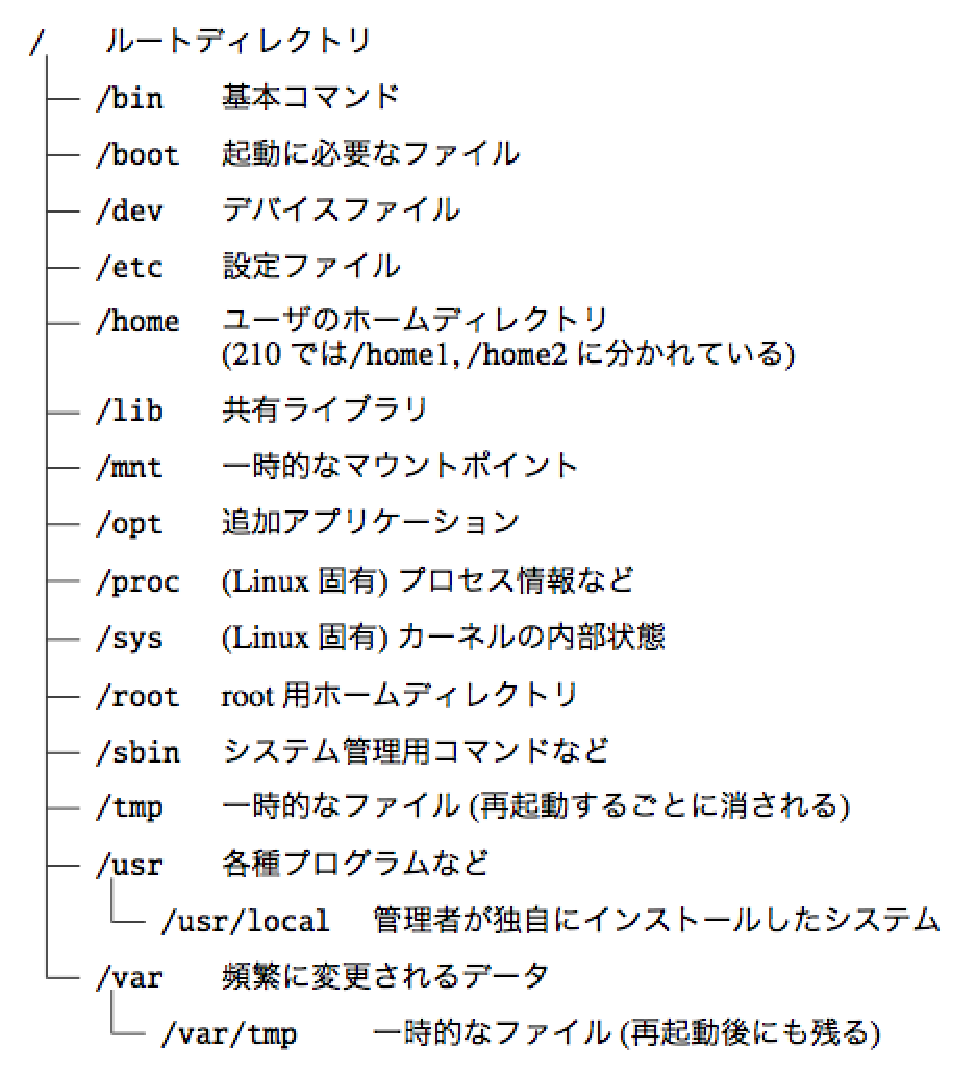
\includegraphics[width=100mm,height=110mm]{Fig/fs-tree2.eps}}
        \caption{UNIX における代表的なディレクトリとその中身}
        \label{fig:dir}
    \end{figure}

    Fig. \ref{fig:dir} を見ると、基本コマンドは\verb+/bin+にあるようです。
    \underline{\texttt{find /bin -name ls}}としてみましょう。
    \begin{screen}
        $\sim$\$ find  /bin  -name  ls\\
        \\
        /bin/ls
    \end{screen}
    とお返事がいただけますね。どうやら\verb+/bin+というディレクトリに\verb+ls+
    が存在しているようです。\verb+head+についても\verb+/bin+にあるのでしょうか。
    同じように\underline{\texttt{find /bin -name head}}としてみましょう。お返事が返ってこな
    いのではないかと思います。こういうときは\underline{\texttt{whereis head}}と入力してみましょう。
    \begin{screen}
        $\sim$\$ whereis  head \\
        \\
        head: /usr/bin/head /usr/bin/X11/head /usr/share/man/man1/head.1.gz
    \end{screen}
    というお返事が返ってくるかと思います。後ろにいろいろと付いているかと思い
    ますが、いまは気にせずに流してください。どうやら\verb+head+は
    \verb+/usr/bin+にあるようですね。Fig 1 を見てみると、\verb+/usr+は
    各種プログラムなどが入っているディレクトリです。ちなみに、
    \underline{\texttt{man whereis}}とすれば分かりますが、\verb+whereis+はコマンドの
    バイナリ・ソース・man ページの場所を示してくれるコマンドです。その他の
    コマンドについても、いくつか試してみましょう。

    \subsection{コマンドはどうやってくるのか?}
    さて、コマンドがどこにいるのかは分かってきました。どうやら\verb+ls+は
    \verb+/bin+というディレクトリにいて、\verb+head+は\verb+/usr/bin+
    にいるようです。試しに、\underline{\texttt{/bin/ls -l}}と入力してみましょう。
    \begin{screen}
        $\sim$\$ /bin/ls  -l 
    \end{screen}

    すると、\verb+ls+と全く同じ出力が得られるはずです。場所さえ知って
    いれば、このように使うことができるのは Windows や Mac OS X などの
    アプリケーションと同じですね。

    しかし、先ほどいくつかのコマンドで確認したように、皆が同じ場所にいるわけ
    ではないようです。にも関わらず、我々はコマンドがどこにいるのかを全く
    知らないまま使うことができています。不思議ですね。この節では、コマンドが
    呼び出される仕組みについて説明します。

    \vspace*{3mm}

    ヒントは、ログイン時に読み込まれるファイル\verb+/etc/profile+にあります。
    起動時のファイル読み込みについては後ほど詳しく説明しますが、
    とりあえず今は中を確かめてみましょう\footnote{ここではsakuraに入った方が下に近い結果を得られるようです。}。
    ターミナル上で\underline{\texttt{less /etc/profile}}と入力してみてください。
    何やら暗号めいた内容が表示されるかと思いますが、一つ一つの解読は
    それぞれの興味にお任せします。各自調べてみたり、TA に聞いてみたりしてみてください。
    ここでは、先ほどからコマンドのありかとして現れている\verb+bin+と
    いう単語を検索してみましょう。\verb+less+による表示内での
    検索をするには\underline{\texttt{/<search term>}} \return~と入力します(つまりスラッシュを打った後探したい言葉を入力する、nと打つと次の検索結果に移る)。この場合、
    \underline{\texttt{/bin}} \return~です。最初の方の\verb+PATH=...+と書かれた箇所を探してください。
    \begin{verbatim}
    if [ "`id -u`" -eq 0 ]; then
      PATH="/usr/local/sbin:/usr/local/bin:/usr/sbin:/usr/bin:/sbin:/bin"
    else
      PATH="/usr/local/bin:/usr/bin:/bin:/usr/games"
    fi
    \end{verbatim}

    このような記述が見つかりましたか?
    さらにこのような記述が最後の方にあったと思います。
    \begin{verbatim}
    export PATH
    \end{verbatim}

    exportはbashにおいて環境変数を設定する
    コマンドです。そしてこの\textbf{環境変数} \verb+PATH+が、
    使えるコマンドの場所を指定しています。
    つまり、いちいちそのコマンドの置き場を指定しなくても、\verb+PATH+で指定されている
    ディレクトリについては自動的に探してくれるということです。
    ``\verb+:+''で区切られて、いくつかのディレクトリが設定されていますが、前に書かれているものほど\textbf{優先的}
    に呼び出されます。つまり、上の例では、仮に\verb+/usr/local/bin/ls+と
    \verb+/bin/ls+が存在していた場合、普通に\verb+ls+と入力したときには
    前の方にある
    \verb+/usr/local/bin/ls+が実行されるということです。環境変数\verb+PATH+において設定
    され、そのディレクトリのコマンドなどをパスの指定なしに利用できる状態のことを
    \textbf{パスが通っている}というような言い方をします。CUI に限らず、
    計算機を便利に利用するためには、パスを通すという概念が非常に重要です。
    現在パスが通っているディレクトリがどうなっているかは、環境変数\verb+PATH+
    を表示する以下のコマンド
    \begin{screen}
    $\sim$\$ echo \$PATH
    \end{screen}
    を実行すれば確認できます。すると、(ちょっと見づらいかもしれませんが)確かに
    \verb+/usr/local/bin:+が入っていることがわかると思います。
    先ほどの\verb+ls+と\verb+head+について、上の\verb+PATH+で確認して
    みましょう。今は下段の方の\verb+PATH+の設定が効いています。確かに\verb+/bin+にも\verb+/usr/bin+にもパスが通って
    いますので、\verb+ls+も\verb+head+も取り立ててパスの指定をすること
    なく利用できていたわけですね。

    ではここで少し試してみましょう。先ほどの\verb+~/exercise+ディレクトリに\verb+line.sh+というコマンドを用意しておきました。
    とりあえず拡張子\verb+.sh+については気にしないでください。これはcatコマンドなど
    で中をみてみれば何となくわかると思いますが、要するに<ファイル名>の<整数>
    行目を抜き出してください、という意味です。
    適当に試してみましょう\footnote{ここはテキストのコピペではなく手打ちの方が上手くいきやすいです。これは$\sim$の微妙な違いによる。}。
    \begin{screen}
        $\sim$\$ \textasciitilde/Unix2\verb+_+Haifu/exercise/line.sh 10  \textasciitilde/Unix2\verb+_+Haifu/exercise/students.txt
    \end{screen}
    お返事がありましたよね?でも
    \begin{screen}
        $\sim$\$ line.sh 10  \textasciitilde/Unix2\verb+_+Haifu/exercise/students.txt
    \end{screen}
    とだけしても、そんなコマンドないよって怒られるはずです。
    たとえ今いるディレクトリに\verb+line.sh+が入っていても
    やはり実行できません。そこで
    \begin{screen}
        $\sim$\$ PATH=\$PATH:\textasciitilde/Unix2\verb+_+Haifu/exercise\\
        \\
        $\sim$\$ line.sh 10  \textasciitilde/Unix2\verb+_+Haifu/exercise/students.txt
    \end{screen}
    としてみましょう。今度は怒られないはず。
    \verb+~/exercise+にパスを通すことにより(これまでのパスに\verb+~/exercise+を追加)
    \verb+line.sh+コマンドが使えるようになったわけです。
    \subsection{環境変数について}
    環境変数について、少しだけ説明しておきます。環境変数とは、その名の通り、
    端末の環境に関する情報です。ターミナルで\underline{\texttt{env}} (environment の略) 
    と入力してみて下さい。
    \begin{verbatim}
    MANPATH=/usr/local/intel/idb/man:/usr/local/intel/ifc/man:/usr/local/intel/icc/man:/usr/local/
    intel/idb/man:/usr/local/intel/ifc/man:/usr/local/intel/icc/man:/usr/local/intel/idb/man:/usr/
    local/intel/ifc/man:/usr/local/intel/icc/man:/usr/local/intel/icc/man:/usr/local/man:/usr/loca
    l/share/man:/usr/share/man
    INTEL_LICENSE_FILE=/usr/local/intel/icc/licenses:/opt/intel/licenses:/home2/koshin/intel/licen
    ses:/Users/Shared/Library/Application Support/Intel/Licenses:/usr/local/intel/ifc/licenses:/op
    t/intel/licenses:/home2/koshin/intel/licenses:/Users/Shared/Library/Application Support/Intel/
    Licenses:/usr/local/intel/icc/licenses:/opt/intel/licenses:/home2/koshin/intel/licenses:/Users
    /Shared/Library/Application Support/Intel/Licenses:/usr/local/intel/ifc/licenses:/opt/intel/li
    censes:/home2/koshin/intel/licenses:/Users/Shared/Library/Application Support/Intel/Licenses:/
    usr/local/intel/icc/licenses:/opt/intel/licenses:/home2/koshin/intel/licenses:/Users/Shared/Li
    brary/Application Support/Intel/Licenses:/usr/local/intel/ifc/licenses:/opt/intel/licenses:/ho
    me2/koshin/intel/licenses:/Users/Shared/Library/Application Support/Intel/Licenses
    TERM=xterm-256color
    SHELL=/bin/bash
    .                                                
    .
    .
    \end{verbatim}

    このようにさまざまな環境変数があります。これらの環境変数が、現在皆さんが
    使っている端末において定義され、端末の環境を規定しているわけです。
    今後色々なアプリケーションをインストールするとき、インストールガイドなどで
    「◯◯という環境変数を設定するように」という指定がなされることがあると思います。
    そのときはここでやったことを思い出してみるとよいでしょう。
    また、興味のある方は、それぞれの意味について調べてみると良いと思います。



    \section{起動のはなし}
    さて、話を本筋に戻しましょう。これまでの話をまとめると、\textbf{コマンド
    は主に /bin や /usr/bin などのディレクトリ内にしまわれており、
    それらのディレクトリにパスを通すことによって、パスを指定しなくてもコマン
    ドが利用できる}という話でした。\textbf{環境変数 PATH は /etc/profile の
    中で定義されていました}。ここまでは良いですね。

    少しずつ、端末の中がどうなっているのかが分かってきましたね。
    しかし、まだ大きな疑問が残っています。
    本来パスの設定などは個人設定として、自分で自由に
    追加したり削除したりしたいところです。
    でも先ほどの
    \verb+/etc/profile+ というディレクトリは、いかにも個人で変えられそうもないところにあります。
    実際に\underline{\texttt{emacs /etc/profile \&}}などとして何か書きかえようとしてみればわかり
    ます。権限がないと怒られるはずです。ではどのようにすれば自分で好きなように
    個人用の環境変数を設定すればよいのでしょうか。
    それを理解してもらうために、この章では、端末の起動の仕組みについて説明します\footnote{使っ
    ているシェルやディストリビューションによって、異なる部分がありますが、
    ここでは559の環境を想定し、典型的な一例を示します。}。

    \subsection{ログイン}
    もう問題無いかと思いますが、ユーザ名とパスワードを入力して、
    端末にログインをします。ここでユーザの認証が行われて、それぞれの
    環境に向かい入れてもらえます。ちなみに現在の 210 はパスワード
    入力時に * が表示されると思いますが、UNIX 系の端末ではパスワードの
    流出を防ぐため、何も表示されないこともあります。ネットワークの
    回で学んだssh を用いて、外部ログインを
    すでに試した人は、ログインするときのパスワード入力のとき何も表示されないことに気づいたと思います。

    \subsection{/etc/profile の読み込み}
    ログインに成功すると、\verb+bash+が起動し、\verb+/etc/profile+が
    読み込まれます。これは全てのユーザに共通の設定ファイルであり、
    ログイン時に一度だけ読み込まれます。

    %\subsection{$\sim$/.profile の読み込み} <= 2022Ver
    %上のように書くと"Token not allowed in a PDF string"という警告が出る
    %(hyperrefに関連する警告らしい, 綿貫は詳細はよく分からず...)
    \subsection{\texorpdfstring{$\sim$/.profile の読み込み}{~/.profile の読み込み}}
    \verb+/etc/profile+の次に読み込まれるのが、ホームディレクトリに
    ある\verb+.bash_profile+\footnote{\texttt{.profile}のような名前になっている場合もあります。}です。
    ホームディレクトリに存在することからも分かるように、このファイルは個人用の設定ファイルです。
    \verb+.bash_profile+も\textbf{ログイン時に一度しか}読み込まれません。
    \verb+/etc/profile+との違いは、\textbf{全ユーザに共通か、
    個人にのみ適用されるか}、という点です。つまり、全ユーザについて設定して
    おくべきことは\verb+/etc/profile+に書き込まれます。

    %\subsection{$\sim$/.bashrc の読み込み}
    \subsection{\texorpdfstring{$\sim$/.bashrc の読み込み}{~/.bashrc の読み込み}}
    次に読み込まれるのが、\verb+.bashrc+です。
    \verb+.bashrc+は\textbf{シェルを起動する毎(ターミナルなどを新たに立ち上げる毎)}
    に読み込まれます。もちろん、これも個人毎の設定ファイルになります。
    \verb+.profile+とのもっとも大きな違いは、\textbf{.bash\_profile
    がログイン時に一度だけ読み込まれるのに対し、.bashrc はシェルを起動するた
    びに読み込まれる}という点です。つまり、一度だけ設定すればよいことは
    \verb+.bash_profile+に書かれ、シェルを起動する毎に設定すべきことが
    \verb+.bashrc+に書かれます。
    先ほどのPATHの設定などは\verb+.bash_profile+と\verb+.bashrc+のどちらに書くことも
    できます.ただ、\verb+.bashrc+の中で設定した方が
    ターミナルを立ち上げ直すだけですぐに変更が反映される(いちいち再ログインしなくてよい)
    ので、そちらの方が一般的です。
    皆さんの場合は
    \begin{verbatim}
    # PATH etc の設定
    export PATH=/usr/local/intel/idb/bin:/usr/local/intel/ifc/bin:
    /usr/local/intel/icc/bin:/usr/local/bin:/usr/bin:/bin:/usr/games
    \end{verbatim}
    などとしておいて\footnote{見やすさのために改行していますが、実際にはこの
    書き方はできません。1行で書くか、改行するところにバックスラッシュを
    付ける必要があります。}
    これに適宜足していくのがよいかと思います。
    また、一度に書かずに
    \begin{verbatim}
    # PATH etc の追加
    export PATH=$PATH:<追加したいパス>
    \end{verbatim}
    などとして、これまでのパスに順次追加することもできます。
    \vspace*{3mm}

    その他にも、\verb+/etc/.profile.d+というディレクトリや、
    \verb+~/.bash_login+、\verb+~/.bash_logout+といったファイルが
    存在する場合もありますが、概ねの流れは 3.1 節から 3.4 節のような感じです。
    Fig \ref{fig:login} に流れを示しておきます。

    \begin{figure}[htbp]
        \centering
        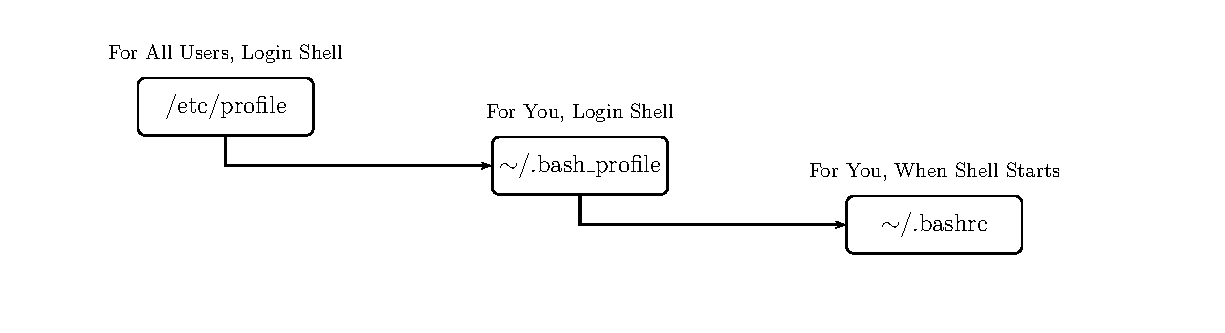
\includegraphics[width=150mm]{Fig/login.eps}
        \caption{ログイン後に読み込まれるファイル}
        \label{fig:login}
    \end{figure}

    また、予想できるかと思いますが、\verb+.bash_history+はコマンドのヒストリ
    機能\footnote{過去実行したコマンドを記憶してくれる機能のこと。}を
    助けるためのファイルです。
    
    \underline{\texttt{less .bash\_history}} で中をのぞいてみ
    ると、皆さんがこれまでに入力したコマンドが並んでいるはずです。

    \subsection{ファイルの中をのぞいてみよう}
    さて、今までに出てきたファイルの中身を少しのぞいてみましょう。

    まず、\verb+/etc/profile+をのぞいてみましょう。
    \underline{\texttt{cat -n /etc/profile}}としてみてください。
    以下はsakuraでの実行例です\footnote{edu端末だと少し違うようです。}。

    \begin{verbatim}  
     1 # /etc/profile: system-wide .profile file for the Bourne shell (sh(1))
     2 # and Bourne compatible shells (bash(1), ksh(1), ash(1), ...).
     3 
     4 if [ "`id -u`" -eq 0 ]; then
     5   PATH="/usr/local/sbin:/usr/local/bin:/usr/sbin:/usr/bin:/sbin:/bin"
     6 else
     7   PATH="/usr/local/bin:/usr/bin:/bin:/usr/local/games:/usr/games"
     8 fi
     9 export PATH
    10 
    11 if [ "$PS1" ]; then
    12   if [ "$BASH" ] && [ "$BASH" != "/bin/sh" ]; then
    13     # The file bash.bashrc already sets the default PS1.
    14     # PS1='\h:\w\$ '
    15     if [ -f /etc/bash.bashrc ]; then
    16       . /etc/bash.bashrc
    17     fi
    18   else
    19     if [ "`id -u`" -eq 0 ]; then
    20       PS1='# '
    21     else
    22       PS1='$ '
    23     fi
    24   fi
    25 fi
    26 
    27 if [ -d /etc/profile.d ]; then
    28   for i in /etc/profile.d/*.sh; do
    29     if [ -r $i ]; then
    30       . $i
    31     fi
    32   done
    33   unset i
    34 fi
    \end{verbatim}

    シェルスクリプトについては、後では触れますが、意味の分かる部分も出てき
    たかと思います。4 行目の\verb+if+はプログラミングをやったことがある人
    なら分かるかもしれませんが、条件によって異なる処理を行う際に用いられる
    構文です。その後の\verb+id+という部分は、\underline{\texttt{man id}}としてみましょう。
    どうやらユーザの情報を参照して、それによって処理を変えているようです。
    ユーザの種類によって、\verb+PATH+の値を変更しているようです。
    \verb+PS1+に関しては、後でもう少し詳しく説明します。
    というように、何となく意味が分かっていくかと思います。
    
    繰り返しになりますが、
    9行目の\verb+export+というのは、シェルスクリプトの中で定義した
    シェル変数を環境変数にするという操作をしています。少しややこしいですが、
    \verb+export+をしないと、代入された値などはそのシェルの中でしか
    定義されたことにならず、\verb+export+が行われることで環境変数と
    して、そのプロセス(ここでは\verb+/etc/profile+が実行されたシェル内)から
    起動されるプロセス(例えば、新たに立ち上げたシェル)にも値が引き継がれる
    ということになります。

    \vspace*{3mm}

    次は\verb+~/.bash_profile+の中をのぞいてみましょう。先ほどと同様、
    \underline{\texttt{cat -n .bash\_profile}}としてください\footnote{これはsakuraでもedu端末でもかまいません。}。
    %(文字化けするときは
    %\underline{\texttt{less /etc/profile | nkf -w }}としてみてください)。

    \begin{verbatim}
     1  # ---- language-env DON'T MODIFY THIS LINE!
     2  # .bash_profile は、ログイン時に実行される。
     3  if [ -f ~/.bashrc ]
     4  then
     5    # ただし、すでに .bash_profile が .bashrc を実行していたら、
     6    # 重複しては実行しない。
     7    if [ -z "$BASHRC_DONE" ]
     8    then
     9      . ~/.bashrc
    10    fi
    11  fi
    12  # ---- language-env end DON'T MODIFY THIS LINE!
    \end{verbatim}

    コメントの通り、\verb+.bash_profile+はログイン時に
    実行されます。3 行目は\verb+.bashrc+が存在するかを確かめる条件文です。
    コメントを付けているので大体分かるかと思いますが、コメント(\# 印)の 5 行
    目と 6 行目に書かれている内容が $7 \sim 11$ 行目に書かれているという感じです。
    \verb+BASHRC_DONE+という環境変数の値によって.bashrcが既に起動されているか否かを
    判定しているようです。
    しかし実はこの部分は役に立っていません。それについては後ほど。

    内容としては、\verb+.bashrc+を実行してね、ということですね。
    皆さんの\verb+.profile+は条件付き(\verb+.bashrc+の有無や、
    すでに実行されたかどうか)で実行するように調整されていますが、
    人によっては、\verb+.profile+の記述は、
    \begin{verbatim}
    source ~/.bashrc
    \end{verbatim}
    のみという人もいます。

    \vspace*{3mm}

    ここまでがログイン時に設定されることです。つまり、もし\verb+.bashrc+とい
    う個人設定ファイルがなくても、\verb+/etc/profile+の中に書かれていたこと
    は設定された状態になるということです。\verb+PATH+や\verb+umask+などの
    基本的な部分はここまでですでに定義されていますね。\verb+.profile+
    を見れば分かるように、別に\verb+.bashrc+が無くても、端末が起動しない
    わけではありません。
    なので、自分が新たにパソコンを使い始める時に\verb+.bashrc+が
    ないからといって焦る必要はありません。
    \verb+.bashrc+は基本的には自分で作るものなので、もしなければ新たに作ればよいというだけです.
    
    \vspace*{3mm}

    \verb+.bashrc+の中での設定は、端末を便利に使う上で非常に重要
    なものばかりです。それでは中をのぞいてみましょう。
    \verb+.bashrc+はそれなりに内容が多いので、今回はその中の一部を説明します。
    行数を利用して説明しますので、\underline{\texttt{cat -n .bashrc | less}} などと
    してください\footnote{もう意味は分かりますよね!}。
    その後、何となく分かるような分からないような記述が続きますが、
    最後までみても先ほどの\verb+BASHRC_DONE+という環境変数が現れないことが分かると思います。
    \verb+.bashrc+を起動したか否かを判断するための変数なのに\verb+.bashrc+の中に記述がない。
    これでは\verb+.profile+でわざわざ重複を避けている意味がありませんね。
    役に立っていないと言ったのはそういう理由です。
    気になる人は
    \begin{verbatim}
    # .bash_profile で使う。
     BASHRC_DONE=1
    \end{verbatim}
    などと足しておけばいいでしょう(別にこれをやらなくても何も問題はありません)。

    $11 \sim 20$ 行目の\verb+PS1+については、後の練習で利用します。
    下に進んでいくと、27 行目からは、\verb+aliases+という名前がみえると思います。
    \begin{verbatim}
    28  if [ -f ~/.aliases ]; then
    29    .  ~/.aliases
    30  fi
    \end{verbatim}
    エイリアスというのは覚えていますか?\footnote{bashなどの
    シェルでは、コマンドに別名をつけて登録することができますが、
    その別名登録の際に使用するコマンドがaliasなのでした。}\verb+.aliases+に関しては後で
    説明しますが、どうやらホームディレクトリ下の\verb+.aliases+の
    存在を確認し、読み込んでいるようです。

    また22行目に書かれている\verb+/etc/bash_completion+はシェルの補完機能
    \footnote{Tab を押すとコマンド名やらファイル名やらが補完される機能。
    ちゃんと使っていますよね。使わないと非常に不便です。}を拡張するためのファイルです。
    補完機能の拡張は端末を便利に使うためには不可欠です。興味があれば、
    中をのぞいてみてください。

    その他、気になる部分は各自調べてみたりしましょう。おそらく、最初に
    自分で設定ファイルを作る際は、ネット上に転がっているファイルを拾って
    きて、カスタマイズしていったり、便利そうな機能をコピペしていくと
    いう形になるのではないかと思います。その時のためにも暗号解読の
    スキルを身に付けておきましょう。

    \subsection{練習}
    \verb+.bashrc+に現れる環境変数を少しいじってみましょう。
    11 行目からの記述に含まれる\verb+PS1+という変数を使って、遊んでみます。
    まずは、\verb+.bashrc+の中身を確認しておきます;
    \begin{verbatim}
    11  # プロンプト。man bash 参照
    12  if [ "$TERM" = "dumb" -o "$TERM" = "emacs" ]; then
    13    PS1='\w\$ '
    14  else
    15    if [ "$UID" = "0" ]; then
    16      PS1='\[\e[41m\]\w\$\[\e[m\] '
    17    else
    18      PS1='\[\e[7m\]\w\$\[\e[m\] '
    19    fi
    20  fi
    \end{verbatim}
    \verb+PS1+はプロンプト(コマンドを打ち込む前に表示される印)
    を定義する変数です。どこのことを言っているのか分からない人も
    いると思いますので、とりあえずターミナル上で次のように入力してみましょう。
    `='の前後に空白などは入れないでください。$>$ の後ろには
    空白を1つくらい入れておいた方が、おそらく幸せです。
    \begin{screen}
        $\sim$\$ PS1='> '
    \end{screen}
    \verb+PS1+とは、これによって形が変わった場所のことです。
    これでは違和感があり使いづらいとなったら
    \begin{screen}
        > source .bashrc
    \end{screen}
    とすれば元に戻せます。
    注意して欲しいのは、「PS1」という変数はexportされていないので、環境変数ではないということです。このことは
    \begin{screen}
        $\sim$\$ env
    \end{screen}
    としてみても、PS1は現れないということから確認できます。

    ここからは少し遊んでみましょう。以下の例を実行してみて下さい。
    また、Table \ref{tab:ps1} にいろいろな情報の参照の仕方を
    まとめました。いろいろと遊んでみましょう。
    \begin{screen}
        $\sim$\$ PS1='\verb+\h +' 
    \end{screen}

    \begin{screen}
        $\sim$\$ PS1='\verb+\h \u \n \d \t +'
    \end{screen}

    元祖ニコちゃんマーク。
    \begin{screen}
        $\sim$\$ PS1='\verb+:-) +'
    \end{screen}

    冷や汗。
    \begin{screen}
        $\sim$\$ PS1='\verb+^^; +'
    \end{screen}
    他にも色々バリエーションはあると思います。色なども設定できます。
    \begin{table}[htbp]
        \centering
        \caption{PS1 で利用できる情報とその表記の例}
        \label{tab:ps1}
        \begin{tabular}{cc} \hline\hline
            表記 & 意味 \\ \hline
            \verb+\h+    &  ホスト名  \\
            \verb+\u+    &  ユーザ名  \\
            \verb+\d+    &  日付  \\
            \verb+\t+    &  時刻(24 時間制)  \\
            \verb+\T+    &  時刻(12 時間制)  \\
            \verb+\w+    &  カレントディレクトリ(フルパス)  \\
            \verb+\W+    &  カレントディレクトリ名  \\
            \verb+\n+    &  改行  \\
            \hline\hline
        \end{tabular}
    \end{table}

    \section{設定ファイルやディレクトリ}
    今までに見てきた設定ファイルは、主にシェルに関わる設定ファイルでした。
    そのほかにもさまざまな設定ファイルが存在し、環境やアプリケーションの
    カスタマイズが行えるようになっています。

    \subsection{.sshディレクトリ}
    \verb|~/.ssh/config|というファイルがSSHの設定ファイルです\footnote{無ければ
    touchコマンドで作ることもできます。
    windowsの場合はtouchコマンドが使えない(らしい)のでnotepadコマンドを試してみてください。}。
    たとえば、
    \begin{Verbatim}[baselinestretch=0.5]
    Host dover
            HostName dover.eps.s.u-tokyo.ac.jp
            User s212601

    Host edu01
            HostName edu01.eps.s.u-tokyo.ac.jp
            User s212601
            ProxyCommand ssh -X dover nc %h %p

    Host www-geoph
            HostName www-geoph.eps.s.u-tokyo.ac.jp
            User s212601
            ProxyCommand ssh -X dover nc %h %p
    \end{Verbatim}
    のように記述しておくと便利です。こうしておけば
    \begin{verbatim}
    $ ssh -X s212601@dover.eps.s.u-tokyo.ac.jp
    \end{verbatim}
    とわざわざ入力しなくても
    \begin{verbatim}
    $ ssh -X dover
    \end{verbatim}
    と入力するだけで済むようになります。
    またeduやwww-geophにログインする場合もdoverに一旦SSHする必要はなく、直接
    \begin{verbatim}
    $ ssh -X edu01
    \end{verbatim}
    とするだけで済みます。SCPやSSHFS\footnote{本テキストでは説明しません。
    リモートマシン上のファイルをローカルのファイルと同じように扱えるため便利なので
    中〜上級者は使ってみてください。}にも有効なのでぜひ設定しましょう。

    \subsubsection{踏み台サーバー}
    計算機演習室のサーバーは、dover以外は学外からsshできない設定になっています。
    そのため、みなさんは毎回最初にdoverにログインしてから更にsshして目当てのサーバーにアクセスする必要がありました。
    世の中にはこのような構成になっているサーバーがたくさんあります。
    こういったサーバーにアクセスする際に毎回2回のsshログインをし2回のexitをするのは手間です。
    これは実は設定ファイルにProxyCommandという1行を書くだけで一発で認証できるようになります。

    \subsubsection{公開鍵認証}
    \verb|~/.ssh/|には\verb|config|以外のファイルも配置されます。
    その中で最も重要なものが、鍵ファイルです。

    これまで皆さんは、SSHで遠隔ログインする際にパスワードの入力を求められてきました。
    これは「背後に人が立っていてパスワードを盗み見られる」といった脆弱性があります。
    また、単純にパスワードを打つのが面倒だという問題もあります。
    そこで、これを解決する方法の一つとして公開鍵認証
    \footnote{暗号化に用いる鍵と復号化に用いる鍵が異なっているもの。
    この場合鍵ペアのうち暗号化に用いるものは公開しても問題ない。}が広く用いられています。

    設定方法は次の通りです。ただし、edu端末のssh環境は少し厄介なようなので、ここでは
    「こうすれば多くの場合上手くいく」といったような一般論を述べたいと思います\footnote{筆者の
    個人用PC(MacBook Air)ではこの方法で上手くいきました。}。

    \vspace*{3mm}

    まず、ローカルホストで \verb|~/.ssh/|へ移動し、%\footnote{eduでは
    %\texttt{/Users/s??????/.ssh}に移動すると良いようです。}
    \begin{screen}
        \texttt{~/.ssh\$ ssh-keygen}
    \end{screen}
    を実行します。すると
    \begin{verbatim}
    Generating public/private rsa key pair.
    Enter file in which to save the key (/home/xxx/.ssh/id_rsa):
    \end{verbatim}
    と表示されるので、鍵の名前を設定します。
    未入力で進むとid\_rsaという名前が自動的に設定されます。
    このテキストでは鍵の名前はid\_rsaとします。

    次に、
    \begin{verbatim}
    Enter passphrase (empty for no passphrase):
    \end{verbatim}
    と表示されます。
    多くの場合は空にしますが、盗難等を心配して鍵を開くためのさらなるパスワードを設定することもできます。
    入力すると確認されるので、同じ文字列を再度入力します。

    すると、\verb|~/.ssh/|に\verb|id_rsa|というファイルと\verb|id_rsa.pub|という2つのファイルが作成されます。
    見ての通り、\verb|id_rsa.pub|が公開鍵ですので、これをサーバーに転送して使います\footnote{注意:
    win端末では ssh-copy-id が使えないようです! win端末からssh-copy-idっぽいことをしたい場合は、例えば
    このQiita記事を参考にしてみてください。\url{https://qiita.com/tabu_ichi2/items/446722c15e6b5678ccad}}。
    \begin{verbatim}
    ssh-copy-id -i ~/.ssh/id_rsa.pub username@hostname
    \end{verbatim}
    とすれば公開鍵がサーバーに転送され適切に配置されます。

    最後に、鍵認証で接続する設定を行います。
    sshコマンドのオプションを用いて
    \begin{verbatim}
    ssh -i id_rsa username@hostname
    \end{verbatim}
    として接続することも可能ですし、\verb|~/.ssh/config|に
    \begin{verbatim}
    Host asano
            HostName asano.eps.s.u-tokyo.ac.jp
            User s212601
            ProxyCommand ssh -X dover nc %h %p
            IdentityFile ~/.ssh/id_rsa
            IdentitiesOnly yes
    \end{verbatim}
    のようにIdentityFile行を追加することによって鍵を指定することも可能です。

    \subsection{.bashrc}
    先ほどから何度も出てきているファイルです。中身は先ほども見ましたので、
    ここでは省略します。

    \subsection{.aliases}
    先日の講義でエイリアスという機能を習いました。良く使うコマンドや
    オプションなどを便利に使うためのショートカットのようなものでしたね、
    \verb+.aliases+は、旧eduでは先ほど見た\verb+.bashrc+の最後の方で読み
    込まれていました。\footnote{bashrc内に直接aliasが書き込まれている場合もあるようです。
    見当たらない場合は新規作成するかbashrcに直接書き込みましょう。}
    中をのぞいてみましょう\footnote{例えばlessコマンド}。
    \begin{verbatim}
    alias	md='mkdir'
    alias	rd='rmdir'
    if [ "$TERM" = "dumb" -o "$TERM" = "emacs" ]; then
      alias	ls='ls -F'
    else
      alias	ls='ls -F --color=auto'
    fi
    alias	lf='ls -F'
    alias	la='ls -a'
    alias	ll='ls -l'
    alias	l.='ls -ld .*'
    alias	rm='rm -i'

    alias   ..='cd ..'

    alias   ggre='firefox http://www.google.co.jp'

    alias	grep='grep --color'
    alias	a2ps='a2psj'
    alias	wl='emacs -nw -f wl'
    alias	kterm='kterm -bg gray30 -fg white -cr yellow'

    if [ -x /usr/bin/xdvi-ja ]; then
      alias	xdvi='xdvi-ja'
    fi

    function xtitle() {
      /bin/echo -e "\033]0;$*\007\c"
    }
    \end{verbatim}

    今回はややこしい部分には触れませんので、エイリアスで定義されている
    コマンドをいろいろと使ってみましょう。\verb+la+や\verb+ll+などは
    すでに使っている人もいるかもしれません。よく使うオプションは
    エイリアスで定義しておくと便利です。また、\verb+mkdir+のエイリアスと
    なっている\verb+md+のように、少し長めのコマンドなどにもエイリアスを
    使うと便利です。一つ上のディレクトリに移動する\verb+..+なども
    使い慣れると必須になります。先ほどの\verb+line+コマンドもエイリアスの中
    で定義してやれば問題なく使えます。エイリアスの意味や効用は分かりましたか?

    \subsection{.emacs}
    そのまんまの名前ですが、Emacs の設定ファイルです。\verb+.bashrc+が
    シェルの起動時に読み込まれるように、\verb+.emacs+は Emacs の起動時に
    読み込まれるファイルです
    %\footnote{\verb+.emacs.el+という設定ファイルがあ
    %る場合は、代わりにこちらが読み込まれます。もしホームディレクトリにこれ
    %があったら、レジュメの\verb+.emacs+を\verb+.emacs.el+と読み替えるか、
    %\%verb+.emacs.el+の名前を変えておくなどしてください。}。
    中をのぞいてみましょう。こちらも長いので、工夫して見てください。

    ファイル内では言語環境などの設定がされていると思います。210 の環境では
    気づきませんが、23 行目、27 行目辺りで特に必要の無いメッセージは表示され
    ないように設定されていたりもします。57 行目からは X で立ち上げたとき
    \footnote{Emacs はターミナル上で立ち上げることも可能です。
    \underline{\texttt{emacs -nw}}としてみましょう。}の設定が書かれており、
    メニューバーなどの表示・非表示もここで扱われています。88 行目からは色の設定が
    されています。120 行目からの記述は、\TeX や Fortran を習うときに
    気にしておくとよいでしょう。

    ちなみに、気づいたかと思いますが、先ほどまでのシェル関連のファイルと違い、
    \verb+.emacs+ではコメントアウトの記号は `;' です。
    他のファイルと同列のように並べましたが、今まで見てきたファイル
    はシェルによって実行されるファイルだったのに対し、\verb+.emacs+は 
    Emacs Lisp という Emacs 用のプログラミング言語で書かれています。
    Emacs Lisp は Emacs Lisp で、語り出すと大変なことになりますので、
    興味のある人は調べてみて下さい。





    \chapter{知っておくと便利なコマンド}

    \section{ファイル転送}
    遠隔ログインを使うようになると、ただログインするだけでなく、ファイルの転送もしたくなります。

    \subsection{SCP}
    ファイルの転送を暗号化するには、SCP (Secure CoPy)
    \footnote{2019年4月よりOpenSSH公式よりSCPは非推奨と宣言されています。
    本講義ではcpコマンドとの類似性から引き続きSCPを用いてファイル転送の説明をしますが、
    余裕のある方は代替であるsftpやrsyncを調べてみてください。}を用います。
    SSHを利用して通信を行う方式なのでセキュアです。
    doverや演習室の端末と自分のパソコン間でファイルをやり取りする場合には
    これを使うことになるので、使用頻度はかなり高いと思います。
    使い方は以下の通りです。

    ローカルからリモートにファイルを送る場合には
    \begin{verbatim}
    $ scp filename1 [username@]hostname:filename2
    \end{verbatim}
    \verb|[username@]| となっているのは、ユーザ名がローカルとリモートで同じ場合に
    \verb|username@| を省略できるということで、SSHの時と同様です。
    例えば、手元にあるレポート課題をdoverに送りたい時は
    \begin{verbatim}
    $ scp report.pdf dover.eps.s.u-tokyo.ac.jp:enshu_report.pdf
    \end{verbatim}
    のようになります。

    反対にリモートからローカルにファイルをとってくる場合には
    \begin{verbatim}
    $ scp [username@]hostname:filename1  filename2
    \end{verbatim}
    とします。さらに、-rオプションをつけると、ディレクトリのコピーもできます。
    recursive(再帰的)のrです。 

    いずれにせよ、「送るもの」を先に指定してから、「送り先」を指定します。
    前回扱ったcpコマンドとよく似ていますね。

    第8章「付録」の「早わかり表」もぜひ参考にしてみてください。

    \vspace{1em}

    \subsection{練習}
    \begin{enumerate}
        \item hoge1.datというファイルをdoverに送り、hoge2.datという名前で保存してください。
        \item 1.で送ったファイルをeduに取ってきて、hoge3.datという名前で保存してください。
    \end{enumerate}

    \subsection{WGET}
    例えば、\url{http://www.eps.s.u-tokyo.ac.jp/access.html}というファイルを
    ダウンロードしたいとき、どのような方法があるでしょうか。
    GUIが好きであればFirefoxで右クリックして保存しても良いですが…CUIも使えるように
    して欲しいですね…。

    このファイルは地球惑星科学専攻の場所のアクセスマップです。
    この地惑専攻のウェブサーバには皆さんのアカウントはありませんからSCPは使えません。
    このような時は\textbf{wget}コマンドを利用すると良いでしょう。
    wgetはWebからファイルをダウンロードするコマンドで、
    HTTP・HTTPS・FTPのプロトコルに対応しています。上の例だと、
    \begin{verbatim}
    $ wget http://www.eps.s.u-tokyo.ac.jp/access.html
    \end{verbatim}
    のようにして使います。
    “-x”オプションを用いれば、ディレクトリ構造を保ってダウンロードできます。つまり、
    \begin{verbatim}
    $ wget -x http://www.eps.s.u-tokyo.ac.jp/access.html
    \end{verbatim}
    とすると、カレントディレクトリに www.eps.s.u-tokyo.ac.jp というディレクトリができ、
    その中に access.html が保存されます。

    また、“-r”オプションを用いれば、指定したページに含まれるリンク先を再帰的に取得できます。

    curlというコマンドでも同じことができますが、詳細については割愛します。

    \vspace{1em}

    \subsection{練習}
    \url{http://www-geoph.eps.s.u-tokyo.ac.jp/~s122621/kadai/index.html}と
    そのページに書かれているリンク先を全てダウンロードしてください。

    \section{テキストフィルター}
    シェルを使って入力されたデータにフィルターをかけて指定した文字列などを検索したり、
    変更を加えて出力したいということがあります。
    ここではそういう時に使用するコマンドの例として検索コマンドgrep, find
    とフィルタリングツールのsed, awk を紹介します。

    \subsection{検索 grep} 
    まず検索コマンドgrep です。ホームディレクトリで、
    \begin{verbatim}
    [1] ~$ ls -a | grep rc
    [2] ~$ grep PATH .bashrc
    \end{verbatim}
    などと打ってみてください。
    [1]においてgrepは標準入力(ファイル名リスト)から`rc' を含む行を検索して表示します。
    [2]は隠しファイル.bashrc 中から`PATH'を含む行を検索して表示します。
    このようにgrepは指定したファイルもしくは標準入力から指定された文字列を含む行のみを出力するコマンドです。
    例えば大量にあるFortranファイルからmoduleを含む行を表示させたい場合、
    \begin{verbatim}
    ~$ grep -n module *.f90
    \end{verbatim}
    などとしてファイルを調べることもできます。
    `-n' は行数も表示させるオプションです。

    検索繋がりで、ファイルが行方不明になった時などに使えるファイル検索コマンドを紹介します。
    以下のコマンドは、s192630さんのホームディレクトリの下にある拡張子がf90 のファイルを検索します。
    実行してみてください。
    \begin{verbatim}
    $ find ~s192630/ -name *.f90
    \end{verbatim}

    \subsection{ストリームエディタsed}
    次はフィルタリングツール sed (stream editor) です。
    %2022ver.では\emph{sed}となっていた. 本来は特別なフォントを使う必要があるのだろうか?
    sed を使うと入力に対して様々なフィルター操作をかけて出力することができます。
    そのうちのいくつかをここで紹介します。
    \begin{longtable}[c]{|p{2cm}|p{6.5cm}|p{8cm}|}
        \hline
        \multicolumn{1}{|c|}{\textbf{コマンド}}&\multicolumn{1}{|c|}{\textbf{説明}}&\multicolumn{1}{|c|}{\textbf{例}}\\
        \hline\hline
        s &文字列の置換& sed 's/置換される文字列/置換する文字列/' \\
        \hline
        p &ある文字列が含まれる行の出力& sed '/ある文字列/p'\\
        \hline
        d &ある文字列が含まれる行の削除& sed '/ある文字列/d'\\
        \hline
        c &ある文字列が含まれる行の置換& sed '/ある文字列/c\textbackslash 置換する文字列'\\
        \hline
    \end{longtable}
    このうち特に置換のコマンドs はよく使いますのでもう少し詳しく見ていきましょう。
    例えばbefore をafter に置換するためには次のようになります。
    (元のファイルは変化しません)
    \begin{verbatim}
    [1] ~$ sed 's/before/after/g' filename
    [2] ~$ something | sed 's/before/after/g'
    \end{verbatim}
    ここではg をつけていますがg をつけると読み込んだ行の中の全ての文字列に対して、
    無い場合は各行の1 つ目のみに対して置換を行います。
    例えば
    \begin{center}
        she sells UMI shells by the UMI shore
    \end{center}
    のUMI をsea に置換したいとしたら二つ目のUMI を置換するためにはg を最後につける必要があります。
    またコマンドにはオプションをつけることができます。
    いくつか紹介すると、操作結果に応じて入力ファイルを上書きする-i、
    二つのコマンドを同時に行うための-e、
    変更を加えた行のみの出力行う-n のオプションなどがあります。
    (注:デフォルトでは読み込んだ全ての行が出力されます。) 
    さらに*、\^、\$、.、などのメタキーを上手に使うことでより細かな操作ができるようになります。
    メタキーの使い方は各自で調べて見てください。

    \subsection{awk}
    最後にawk です。
    これは1 つの言語ですのでおよそありとあらゆることができますが、簡単な使い方を紹介します。
    基本構文はsed と同じです。
    \begin{verbatim}
    [1] ~$ awk '{命令}' filename
    [2] ~$ something | awk '{命令}'
    \end{verbatim}
    ファイルの中身または標準入力に対して、1行ずつ'' 内で指定した処理を行います。

    例を見ていきましょう。
    先ほどの`ls -l' でユーザ名とファイル名だけを表示させたい場合、
    つまり各行の3要素めと8 要素目を表示させるには、
    \begin{verbatim}
        ~$ ls -l | awk '{print $3,$8}'
    \end{verbatim}
    と打ちます。
    print はFortran のwrite (*,*) やPythonのprint()に対応します。
    \verb+$3+ は3 要素目という意味です。
    うまくいきましたか?次に先ほどの出力の1 行目を見てみましょう。
    空行が出ています。
    これは入力の1 行目がファイル容量の合計`total \#' であるため、要素数が2 つしかないからです。
    3 要素目と8 要素目は空だとして空行を出力します。
    これに対処するには
    \begin{verbatim}
    ~$ something | awk ' 条件{命令}'
    \end{verbatim}
    という構文を使います。
    各行に対して条件が当てはまるか検討し、当てはまれば命令を実行します。
    試しに次の2 つを実行してみてください。
    \begin{verbatim}
    [1] ~$ ls -l | awk 'NR>1{print $3,$9}'
    [2] ~$ ls -l | awk 'NF>2{print $3,$9}'
    \end{verbatim}
    のいずれも1 行目の空行を出力しないでくれると思います。
    NR は現在の行数、NF は現在の行の要素数を表します。
    行数が1 行目より後のとき実行せよ、または、要素数が2 個より多いとき実行せよという意味です。

    \section{四則演算expr}
    簡単な整数の計算をするコマンドexpr の紹介です。
    \begin{verbatim}
    ~$ expr 1 + 2
    \end{verbatim}
    のようにして使います。
    +、-、\*、/、\% がそれぞれ足し算、引き算、かけ算、割算、余りに対応します。
    空白は必須なので注意してください。





    \chapter{シェルスクリプト}
    \section{シェルスクリプト始めの一歩}

    % ここからいよいよシェルスクリプトについて学びます。
    シェルスクリプトとは、シェルで実行するコマンドを一つにまとめたファイルのことです。
    複数のコマンドを用いるとき、その途中で1箇所でも間違えてしまうと、
    最初からやり直しということにもなりかねません。
    % そのような手間を軽減するために、行いたい作業を1つのファイルにまとめておき、
    % 修正するときはコマンド1つで、ファイル内の作業をすべて実行できるような環境を整えておくと便利ですね。
    % gnuplotのpltファイルに似たものとも考えられます。
    そのような手間を軽減するために、行いたい作業を1つのファイルにまとめておき、
    コマンド1つでファイル内の作業をすべて実行できると便利ですね。
    次の講義で扱うgnuplotのpltファイルに似たものとも考えられます。
    % この章では、ものすごく簡単なシェルスクリプトを、少し時間をかけて説明していきます。
    % 始めは簡単なもので「しくみ」を理解するのが何よりも大切です。

    % \subsection{とりあえずいじりましょう}
    \subsection{Hellow World!}

    ここから配付したサンプルファイルを使っていきます。さっそくsample01.shを見てみましょう。
    \lstinputlisting[caption=sample01.sh]{./sample01.sh}

    たった2行しかありませんがこれも立派なシェルスクリプトです。次のコマンドによって、実行することができます。
    \begin{lstlisting}[numbers=none]
    ~$ sh sample01.sh
    Hello world!
    \end{lstlisting}

    % 今いるディレクトリの中身が表示されるはずです。
    % 今いるディレクトリの中身を表示するコマンドは\texttt{ls}でしたね。
    % このsample01.shというスクリプトは\texttt{ls}と同じ働きをしていることになります
    % \footnote{もしかしたらlsをls -alなどにエイリアスしている人もいるかもしれませんが、
    % シェルスクリプトではエイリアスは機能しません。(もしエイリアスが機能したらとても危険!)}。

    ここで、\texttt{ls -l}をして、sample01.shの詳細情報を見てみましょう。
    \begin{lstlisting}[numbers=none]
    ~$ ls -l sample01.sh
    -rw-r--r-- 1 s212600 20000 29 Jun  9 13:48 sample01.sh
    \end{lstlisting}

    続いてコマンドライン上に次のようにタイプしてみましょう。
    \begin{lstlisting}[numbers=none]
    ~$ ./sample01.sh
    -bash: ./sample01.sh: Permission denied
    \end{lstlisting}

    エラーが出てしまい、実行できませんでしたね。そこで次のコマンドを実行してみてください。
    \begin{lstlisting}[numbers=none]
    ~$ chmod +x sample01.sh
    \end{lstlisting}

    \texttt{chmod}は、\emph{ファイルの権限を変えるコマンド}でしたね。もう一度、詳細情報を見てみましょう。
    \begin{lstlisting}[numbers=none]
    ~$ ls -l sample01.sh
    -rwxr-xr-x 1 s212600 20000 29 Jun  9 13:48 sample01.sh
    \end{lstlisting}
    などと表示され、ファイルの属性が変わっていることがわかりますね。(各権限にxが加わりました)。
    \texttt{chmod}に\texttt{+x}というオプションをつけることで、
    sample01.shというファイルに\emph{実行権}を与えることができます。
    % ところで実行権とは何でしょうか。それは、次のようにするとわかります。
    \begin{lstlisting}[numbers=none]
    ~$ ./sample01.sh
    Hello world!
    \end{lstlisting}
    先ほど\verb| sh sample01.sh |としたときと同じ結果が得られたのではないかと思います。
    実行権を与えるというのは、\emph{それ単独で動くようにする}(shコマンドは必要ない)ということです。
    \footnote{Fortranで、\texttt{gfortran}でコンパイルした後に実行ファイルに対して\texttt{chmod}で実行権を与えなくても
    \\
        \texttt{~\$ ./a.out}
    \\
    で実行できるのは、すでに\texttt{gfortran}によって\texttt{a.out}に実行権が与えられているからです。}。

    % \subsection{もう少しまじめに解説}
    % sample01.shを実行すると\texttt{ls}したときと同じ結果が得られたということは、このシェルスクリプトの本体は2行目であることがわかりますね。ためしにこのスクリプトに1行付け加えて
    sample01.shに1行付け加えてみましょう。
    \begin{lstlisting}[caption=sample01.sh改]
    #!/bin/sh
    echo Hello World!
    pwd
    \end{lstlisting}

    \begin{lstlisting}[numbers=none]
    ~$ ./sample01.sh
    Hello World!
    (今いるディレクトリの絶対パス)
    \end{lstlisting}
    となるはずです。追加された3行目に対応する出力は、普通にターミナルから\texttt{pwd}と入力したときと同じものです。

    以上のことから、\emph{シェルスクリプトは、単にコマンドを並べればよい}ということがわかりますね。
    % どうですか?難しいですか?まだ簡単だね。

    \subsection{1行目について}
    % 順番が逆になりましたが、1行目の説明をしましょう。
    % と言いながらも、今は、1行目はおまじないだと思っていて良いです。
    % それでも気になる人は、以下の説明を読んでください。
    シェルスクリプトの1行目の
    \begin{lstlisting}
    #!/bin/sh
    \end{lstlisting}
    は、"Shebang"(シバン/シェバン)と呼ばれるものです。

    % \begin{quotation}
    ファイルの1行目の行頭が\texttt{\#!}の場合は、そのファイルの実行をカーネル(Unixの中核)に要求します。
    カーネルは\texttt{\#!}のあとの絶対パスで指定されるファイル名を見て、そのファイルをプログラムとして起動します。そして、2行目以降に書いてある内容をそのプログラムの入力とします。
    つまり、このルールからすればシェルスクリプトに限定された書き方ではなく、例えば
    \begin{lstlisting}
    #!/usr/bin/gnuplot -persist
    plot sin(x)
    \end{lstlisting}
    というファイルを作って実行したときには、gnuplotで描かれた$\sin x$のグラフが現れるわけです
    \footnote{筆者の環境では、gnuplotは/usr/bin/gnuplotにあるそうなので、これで通りました。
    bad interpreter: No such file or directoryというエラーが出るときには、
    gnuplotのパスが異なる可能性があります。
    which gnuplotでgnuplotのパスを調べて、適宜書き換えてください。}。
    (\texttt{persist}はgnuplotの、グラフを画面に残しておくというオプションです。)
    % このことから、シェルはカーネルと人間とのやり取りを仲介する存在で、
    % それはまるで、シェルがカーネルを取り囲み、人間との直接的なやり取りを阻んでいる殻のような存在であることから、
    % シェル(殻)と呼ばれるそうですよ。
    % \end{quotation}

    % \subsection{まとめ}
    % とりあえずシェルスクリプトを書きたいと思ったら、
    % \begin{enumerate}
    %  \item Emacsやviなど、適当なエディタでファイルを作成する。拡張子は何でも良いが、Bシェルスクリプトであることを明示的に表すために.shとすることが多い。このとき、必ず1行目は
    % \begin{lstlisting}
    %  #!/bin/sh
    % \end{lstlisting}
    % とする。
    %  \item 2行目以降は、1行に一つずつ、実行したいコマンドを書いていく。
    %  \item \underline{\rm chmod\,\,+x\,\,[ファイル名]}として、ファイルに実行権を与える。
    %  \item \underline{\rm ./ファイル名}として、実行する。
    % \end{enumerate}
    % とすればよいでしたね。なお、実行権を与えずに、$<$\texttt{sh [ファイル名]}$>$としても実行できました。

    % いろいろ誤魔化しもあって、例えば1行に2つ以上のコマンドを書くこともできますし(後述します)、
    % 拡張子が.shでないことも多いのですが、とりあえずはこれでOKです。

    % \subsection{練習その1}
    % とりあえずここまでの練習です。
    \begin{itembox}[l]{\textbf{練習問題1}}
        \begin{itemize}
            \item[(1)] sample01.sh(改)の4行目以降に、好きなコマンドを入力・保存して、実行してみましょう。
            \item[(2)] さらに、次の2行を加えて保存・実行してみてください。
            \begin{lstlisting}[numbers=none]
                cd ..
                pwd
            \end{lstlisting}
            全部の実行が終わった後でもう一度ターミナルに\texttt{pwd}と入力し、自分がいまどこにいるのかを確かめてください。どんなことがわかりますか?
        \end{itemize}
    \end{itembox}

    \newpage
    \section{シェルの基本機能とシェルスクリプト}
    % 先ほどの例ではあまりにやさしすぎて、実用上何の意味もないように見えます。
    % この節からはもう少し実践的にしてみましょう。
    先ほど勉強したシェルの基本機能をシェルスクリプトでも使ってみましょう。

    \subsection{シェル変数}
    % まずはシェル変数です。シェルの中でもFortranのように変数を定義することができます。
    % さっそくシェル変数を使ったシェルスクリプトを見てみましょう。

    % \subsubsection{値の参照 その1}

    \lstinputlisting[caption=sample02.sh]{./sample02.sh}

    実行権を与え、実行してみましょう。
    \begin{lstlisting}[numbers=none]
    ~$ ./sample02.sh
    inko
    fukuro
    
    nakuinko
    
    nakufukuro
    fukuronaku
    \end{lstlisting}

    実行結果は理解できるでしょうか?

    \texttt{\$TORI3}は未定義の変数です。
    Fortranでは、\texttt{implicit none}と書いておけば未定義の変数があってもgfortranに怒られてコンパイルエラーになりました。
    しかしシェルスクリプトでは未定義の変数はnull値で勝手に初期化され、エラーにはなりません。
    従って、シェルスクリプトでは変数に注意してコーティングする必要があります。
    また\texttt{\$TORI1naku}も未定義の変数とみなされました。
    このような場合、変数名を明示的に\texttt{\$\{\quad\}}で囲む必要があります。

    % 下のようになりましたか?(No such file or directoryが出た人は、実行権限があるか確かめてくださいね)。
    % \begin{lstlisting}[numbers=none]
    %  chibutsu
    %  (何も表示されない行)
    %  geoph
    % \end{lstlisting}
    % 1行ずつ追って見てみましょう。sample02.shの2行目で変数\texttt{gakka1}にchibutsuが格納されているので、
    % 5行目は$<$\texttt{echo chibutsu}$>$となって、結局ターミナルにchibutsuが返ってきた、ということです。
    % 同様に7行目も問題ないですね。

    % 6行目はどうでしょう?
    % $<$\texttt{echo gekka1}$>$となっていますが、残念ながら変数\texttt{gekka1}は定義されていません。
    % Fortranではこんなことをすると「そーだ変数なかっぺ。このごじゃっぺが!」と怒られるわけですが、
    % シェルでは新しい変数を見つけると自分で定義しなくても勝手に定義されるので、ここでは何のエラーも出ません。ただ、実際問題として表示された\texttt{gekka1}という変数には何も格納されていないのでそこのところが少し気になります。

    % 実はシェルでは、何も格納されていない段階ではそのシェル変数はヌル(null)値で初期化されています。
    % すなわち6行目は「\texttt{echo }(このあと何もなし)」と展開されるのです。結局sample02.shの5-7行目は

    % \begin{lstlisting}[firstnumber=5]
    %  echo chibutsu
    %  echo
    %  echo geoph
    % \end{lstlisting}
    % となるので、ターミナルには
    % \begin{lstlisting}[numbers=none]
    %  chibutsu

    %  geoph
    % \end{lstlisting}
    % と返ってきたわけです。

    % \subsubsection{値の参照 その2}
    % 先ほどのsample02.shを、次のように変更しましょう。
    % とりあえずシェル変数\texttt{gakka1}のほうだけを使うことにしましょう。

    % \begin{lstlisting}[caption=sample02.sh 改]
    %  #!/bin/sh
    %  gakka1=chibutsu
    %  gakka2=geoph

    %  echo $gakka1_dayo
    %  echo ${gakka1}_datoyo
    % \end{lstlisting}

    % これを保存して実行すると、次のようになります。
    % \begin{lstlisting}[numbers=none]
    %  (何も表示されない行)
    %  chibutsu_datoyo
    % \end{lstlisting}
    % 5行目は\texttt{gakka1\_dayo}全体を一つの変数とみなして、この変数には値が格納されていないので何も
    % 返しません(nullが返されます)。これに対して、6行目は\texttt{\$\{gakka1\}}と、
    % 中カッコでくくることによってシェル変数の範囲を明示的に示しています。
    % こうすることによって変数\texttt{gakka1}の中身がきちんと出てきて、
    % 結局6行目は$<$\texttt{echo chibutsu\_datoyo}$>$となるので、
    % \texttt{echo}の引数の部分が返ってきているということになります。

    % このようにシェル変数を参照する場合、
    % \texttt{\$変数名}あるいは\texttt{\$\{変数名\}}という書き方をすれば良いわけです。

    % \subsection{バッククォート}
    次のサンプルプログラムです。
    \lstinputlisting[caption=sample03.sh]{./sample03.sh}

    実行してみると、あなたのユーザ名が標準出力に出てきたはずです。

    バッククォート`\quad`(日本語キーボードではShift$+$@、USキーボードでは1キーの左隣)
    または\texttt{\$(\quad)}を用いて、変数にコマンドの実行結果を代入することができました。

    % これはどういうことかというと、2行目で変数\texttt{name}に、
    % コマンド\texttt{whoami}で標準出力に出力される出力結果(つまり、あなたのユーザ名)が格納されます。
    % バッククォート(日本語キーボードではShift$+$@、USキーボードでは1キーの左隣)で囲まれた部分のコマンドは、
    % その実行結果に置換されます。
    % コマンドをクォーテーション(`\,\,')で囲んでいるのではなく、両方とも`であることに注意してください。

    % \subsection{パイプとリダイレクト}
    % シェルスクリプトの中でパイプとリダイレクトも使えます。
    % この辺まで来るとようやくシェルスクリプトを書くありがたみがわかってきます。さっきの
    sample03.shを次のように書き換えてみましょう。
    % (2行目の\texttt{rev}ってのは、出力をひっくり返すコマンドです)。
    \begin{lstlisting}[caption=sample03.sh 改]
    #!/bin/sh
    name1=`echo I am \`whoami\`.`
    name2=$(echo I am $(whoami).)
    echo ${name1}
    echo ${name2}
    \end{lstlisting}

    実行すると、例えばユーザ名が\texttt{s212600}のひとは、
    \begin{lstlisting}[numbers=none]
    ~$ ./sample03.sh
    I am s212600.
    I am s212600.
    \end{lstlisting}
    と返ってくるはずです。
    % ポイントは2行目で、
    % \begin{itemize}
    %  \item \texttt{whoami}の出力結果(あなたのユーザ名)が
    %  \item \texttt{echo}の引数になり、結局\texttt{echo (ユーザ名)}となり、
    % その出力結果(しつこいけどユーザ名)が
    %  \item \texttt{rev}の標準入力になる
    % \end{itemize}
    % ことによって、ユーザ名がひっくり返ったものが変数\texttt{name}に入ったわけです。ただし
    2行目で、`の前にエスケープシーケンスがついているのは、メタキャラクタと区別するためです。
    3行目の書き方ではエスケープシーケンスは必要ありませんね。

    ssh先にリダイレクトすることもできます。先ほど改めたsample03.shをdoverに投げる場合は、このようにします。
    \begin{lstlisting}[numbers=none]
    ~$ ssh dover < sample03.sh
    I am s212600.
    I am s212600.
    \end{lstlisting}
    このように返ってくるはずです。

    % \subsection{練習その2}
    % sample03.shをさらに書き換えて、
    % \begin{lstlisting}[caption=sample03.sh 改2]
    %  #!/bin/sh
    %  name=`echo \`whoami\` | rev`

    %  echo ${name} > revname.txt
    % \end{lstlisting}
    % とすると、4行目でリダイレクトしているのでユーザ名がひっくり返ったものが
    % revname.txtというファイルに書き込まれているはずです。まずはこれを確認してください。

    さらに次のように書き換え、sample04.shとします。
    \begin{lstlisting}[caption=sample04.sh]
    #!/bin/sh
    name1=`echo I am \`whoami\`. | rev`
    name2=$(echo I am $(whoami). | rev)
    filename=revname.txt
    echo ${name1} > ${filename}
    echo ${name2} >> ${filename}
    \end{lstlisting}

    % これはどうなりますか?さらにさらに、
    % \begin{lstlisting}[caption=sample03.sh 改4]
    %  #!/bin/sh
    %  name=`echo \`whoami\` | rev`
    %  filename=`wc -l sample01.sh`

    %  echo ${name} > ${filename}.txt
    % \end{lstlisting}
    % の結果は説明できますか?頭の体操のようになってきましたね。
    % (\texttt{wc}コマンドとそのオプションがわからない人は自分でググってみましょう)。

    \begin{itembox}[l]{\textbf{練習問題2}}
        sample04.sh を作成・実行して、出力ファイルの内容を確認してください。
    \end{itembox}

    % \subsection{四則演算}
    % 前回使った、\texttt{expr}コマンドを使うとシェルスクリプトで計算もできます。
    % サンプルプログラムsample04.shは、この演算子の使い方の例を示したものです。
    % \lstinputlisting[caption=sample04.sh]{./sample04.sh}
    % 算術演算子の部分には、以下の表に示すような演算子が使えます。残念ながら浮動小数点は扱えません。

    % \begin{center}
    % \begin{longtable}{|c|l|}
    % \hline
    % \multicolumn{1}{|c|}{\textbf{算術演算子}}&\multicolumn{1}{|c|}{\textbf{説明}}\\
    % \hline\hline
    % 値1 $*$ 値2 & 値1と値2の積 \\
    % \hline
    % 値1 $/$ 値2 & 値1$\div$値2の商 \\
    % \hline
    % 値1 $\%$ 値2 & 値1$\div$値2のあまり \\
    % \hline
    % 値1 $+$ 値2 & 値1と値2の和 \\
    % \hline
    % 値1 $-$ 値2 & 値1と値2の差 \\
    % \hline
    % \caption{算術演算子の一覧}
    % \end{longtable}
    % \end{center}

    % \subsection{引数をとるスクリプト}
    % これまではシェルスクリプトのファイル名を入力すると、
    % 何か動作をして結果を返してくるだけのシェルスクリプトを考えてきました。
    % でもこれではちょっと限界があって、やはり引数をとって、
    % それによって振る舞いが変わるようなスクリプトも書きたいものです。
    % 引数というのは$<$\texttt{echo 1}$>$というときの\texttt{1}とか、
    % $<$\texttt{seq 1 1 5}$>$のときの\texttt{1}と\texttt{1}と\texttt{5}のようなものです。
    % ここに何を書くかによって、振る舞いが変わってきますね。

    % それで、普通の状態ではシェルスクリプトは9つまでの引数をとることができます。
    % 引数はシェルスクリプトの中で\$1,...,\$9と表わされ、この順番に参照されます。
    % (つまり1つ目にコマンドラインから渡した値は\$1として扱われます)。
    % \$*とすると全ての引数を一度に参照できます。
    % また、\$0にはスクリプトが呼び出された時の名前が入っています。

    \subsection{特殊変数}
    シェルスクリプトには、特殊変数と呼ばれる特別な変数があります。
    \begin{longtable}[c]{|c|l|}
        \hline
        \multicolumn{1}{|c|}{\textbf{特殊変数}}&\multicolumn{1}{|c|}{\textbf{説明}}\\
        \hline\hline
        \texttt{\$0} & シェルスクリプトの名前 \\
        \hline
        \texttt{\$1,\$2,...\$9} & シェルスクリプトの1番目,2番目...9番目の引数 \\
        \hline
        \texttt{\$\#} & シェルスクリプトの引数の数 \\
        \hline
        \texttt{\$*} & シェルスクリプトの引数全部 \\
        \hline
        \texttt{\$@} & シェルスクリプトの引数全部 \\
        \hline
        \caption{シェルスクリプトの特殊変数}
    \end{longtable}

    % \subsection{練習その3}
    % まずはsample04.shをいろいろいじってみてください。
    % ある程度慣れたら次のようなsample05.shを自分で作ってみてください。
    特殊変数を用いて、引数をとることができます。\texttt{expr}は整数の四則演算をするコマンドです。
    \lstinputlisting[caption=sample05.sh]{./sample05.sh}
    % 2行目で\$1と\$2という表現が出てきています。
    % これが「引数をとるスクリプト」の例で、このsample05.shは、数字の引数を2つ必要とします。
    % つまり、実行する際は
    \begin{lstlisting}[numbers=none]
    ~$ ./sample05.sh 5 10
    15
    \end{lstlisting}
    のように実行すると上手く動きます。
    引数の値は自由に変えてみてください。
    また、2行目を\texttt{echo `expr \$1+\$2*\$3`}などとしていろいろ遊んでみてください。
    ちなみに\$3まで使えば、当然引数は3個必要です。

    ところで、シェル変数には型の概念がないことは前に説明しました。
    5や10のような数は整数として適宜判断してくれています。ためしに同じsample05.shを
    \begin{lstlisting}[numbers=none]
    ~$ ./sample05.sh carrot eggplant
    \end{lstlisting}
    のように実行してみるとどうなりましたか?

    \subsection{ヒア・ドキュメント}
    またまたサンプルファイルです。
    \lstinputlisting[caption=sample06.sh]{./sample06.sh}

    % おそらくこのようなお返事が返ってくるでしょう。
    \begin{lstlisting}[numbers=none]
    ~$ ./sample06.sh 
    set terminal pdfcairo
    set output 'sin.pdf'
    plot sin(x)
    \end{lstlisting}

    これは2行目の\texttt{<<EOF}から6行目の\texttt{EOF}の間に書かれている内容がそのまま\texttt{cat}の標準入力に渡されて、
    \texttt{cat}の標準出力にこれが出力されたというわけです。
    このような機能をヒア・ドキュメントといいます。

    これをみているといかにもgnuplotのコマンドですね。
    もう少し解説します。
    シェルは\texttt{<<}というマークを見つけると、それに続く文字列(今の場合は\texttt{EOF})を覚えて、
    次に同じ文字列が出てくる直前の行までをその前のコマンドの標準入力に渡します。
    実は\texttt{EOF}でなくても、\texttt{orz}でも\texttt{SHIROHARAINKO}でも何でも良いわけです(記号文字は不可)。
    \texttt{EOF}というのは``End of File''の略で、一般的には\texttt{EOF}が使われます。
    (渡したい文字列に"EOF"が含まれる場合は、当然\texttt{EOF}以外にする必要があります。)

    もう一つ大事なこととして、ヒア・ドキュメントの中では変数が展開されます。
    つまり、sample06.shを少し書き換えて、このようにしてみましょう。
    \begin{lstlisting}[caption=sample06.sh 改]
    #!/bin/sh
    number=1
    cat <<EOF
    set terminal pdfcairo
    set output 'sin${number}.pdf'
    plot sin(${number}*x)
    EOF
    \end{lstlisting}
    シェル変数\texttt{number}の部分が展開されて、
    \begin{lstlisting}[numbers=none]
    ~$ ./sample06.sh 
    set terminal pdfcairo
    set output 'sin1.pdf'
    plot sin(1*x)
    \end{lstlisting}
    と返ってきます。

    さていよいよ、\texttt{cat}の部分を\texttt{gnunplot}に変えて実行してみましょう。
    ヒア・ドキュメントの中身がそっくりそのままgnuplotに渡されて、
    $\sin x$のグラフがsin1.pdfというファイルに書かれたはずです。

    ここまでくれば、シェルスクリプトもかなり便利なものになってきたのではないでしょうか?

    \section{シェルスクリプトの制御文}
    % この節では、たくさんの絵を一度に作りたいときなどに便利な方法を紹介します。

    \subsection{ループ制御:for文}
    Fortranのdoループのようなこともできます。
    ただし、表式はだいぶ違います。
    例えば指定された回数だけコマンドを実行するような場合、for文が使えます。
    構文は次のような感じです。
    \begin{lstlisting}
    for 変数 in 引数1 引数2 引数3 ...
    do
        コマンド
    done
    \end{lstlisting}
    サンプルも使ってみましょう。
    \lstinputlisting[caption=sample07.sh]{./sample07.sh}
    実行してみると、、、
    \begin{lstlisting}[numbers=none]
    ~$ ./sample07.sh 
    1
    2
    3
    4
    5
    \end{lstlisting}
    となりましたか?要するに、2行目の\texttt{in}の後ろに並んだ引数が順番に変数の部分に入って、
    あとはdoとdoneで囲まれた部分が、引数が空になるまで繰り返されるということです。

    別に\texttt{in}の後ろは数字でなくても構いません。この辺はFortranより自由な感じですね。例えば、
    \begin{lstlisting}[caption=sample07.sh 改]
    #!/bin/sh
    for i in sekiseiinko kozakurainko okameinko
    do
    echo ${i}
    done
    \end{lstlisting}
    などと書いておけば、たくさんの鳥を出力することができます。

    話を戻して、\texttt{in}のあとに先ほど学んだバッククォートによるコマンド置換を使ってみることにします。
    ターミナルで
    \begin{lstlisting}[numbers=none]
        ~$ seq 1 1 5
    \end{lstlisting}
    としてみてください。
    \begin{lstlisting}[numbers=none]
    1
    2
    3
    4
    5
    \end{lstlisting}
    と返ってくるはずです。ということは先ほどのsample07.shの2行目の\texttt{in}のあとを
    \begin{lstlisting}[caption=sample07.sh 改2]
    #!/bin/sh
    for i in `seq 1 1 5`
    do
    echo ${i}
    done
    \end{lstlisting}
    などとすれば、\texttt{in}のあとに\texttt{1 2 3 4 5}と書いたのと同じことになるわけです。
    引数が5つくらいであれば別にありがたみを感じませんが、1から100までとかになれば効果覿面ですよ。

    またbashでは、C言語風に次のように書くこともできます。
    \begin{lstlisting}[caption=sample07.sh 改3]
    #!/bin/sh
    for (( i=1 ; i <= 5 ; i++ ))
    do
    echo ${i}
    done
    \end{lstlisting}

    % \subsection{練習その4}
    % sample06.shとsample07.shをくっつけて、以下のようなファイルsample08.shを作ってみましょう。
    % \begin{lstlisting}[caption=sample08.sh]
    %  #!/bin/sh
    %  for i in `seq -f %02g 1 1 5`
    %  do
    %  gnuplot <<EOF
    %  set terminal postscript color eps enhanced
    %  set output 'sin${i}.eps'
    %  plot sin(${i}*x)
    %  EOF
    %  done
    % \end{lstlisting}
    % どうなりましたか?(seqコマンドのfオプションが何を表しているのか、\%02gが何を表しているのかは自分で調べてみましょう。(最後の課題にも関係していたりいなかったり)

    \begin{itembox}[l]{\textbf{練習問題3}}
        sample06.shとsample07.shを参考にして、$\sin(x), \sin(2x), ... \sin(5x)$のグラフをそれぞれsin1x.pdf, sin2x.pdf, ... sin5x.pdfに出力するシェルスクリプトsample08.shを作ってください。
    \end{itembox}

    \subsection{ループ制御:while文}
    for文の他に、while文によるループの書き方もあります。\texttt{while}の後の条件式が真である間、実行され続けます。
    \begin{lstlisting}[caption=sample07.sh 改4]
    #!/bin/sh
    i=1
    while [ ${i} -le 5 ]
    do
    echo ${i}
    i=$(expr ${i} + 1)
    done
    \end{lstlisting}
    無限ループも作れます。\texttt{break}でループを抜けます。(if文は次節を参照)
    \begin{lstlisting}[caption=sample07.sh 改5]
    #!/bin/sh
    i=1
    while true
    do
    echo ${i}
    if [ ${i} -eq 5 ]
    then
        break
    fi
    i=$(expr ${i} + 1)
    done
    \end{lstlisting}
    
    \subsection{条件分岐:if文}

    シェルスクリプトでもif文が使えます。使い方は次のとおりです。
    \begin{lstlisting}
    if 条件式1
    then
    条件式1が真のときに実行される命令
    elif 条件式2
    then
    条件式1が偽で条件式2が真のときに実行される命令
    elif 条件式3
    then
    条件式1と条件式2が偽で条件式3が真のときに実行される命令
    ...
    else
    すべての条件式が偽のときに実行される命令
    fi
    \end{lstlisting}
    \texttt{if}が\texttt{fi}で終わるあたりに遊び心を感じますが、Fortranに似ていますね。
    \texttt{elif}なのにも注意が必要です。よく間違えます。
    条件式の部分は大カッコ+空白( \verb*|[ |)と、空白+大カッコ( \verb*| ]| )でくくる必要があり、表8に示すようなものがあります。
    始めのカッコの直後と終わりのカッコの直前に空白が必要なことに注意してください。

    \begin{center}
        \begin{longtable}{|c|l|}
            \hline
            \multicolumn{1}{|c|}{\textbf{条件式}}&\multicolumn{1}{|c|}{\textbf{真になる条件}}\\
            \hline\hline
            [ 文字列1 = 文字列2 ] & 文字列1と文字列2が同じ \\
            \hline
            [ 文字列1 != 文字列2 ] & 文字列1と文字列2が同じでない\\
            \hline
            [ -n 文字列 ]  & 文字列が空でない(not zero) \\
            \hline
            [ -z 文字列 ]  & 文字列が空(zero) \\
            \hline
            [ 整数1 -eq 整数2 ] & 整数1と整数2は等しい(equal) \\
            \hline
            [ 整数1 -ge 整数2 ] & 整数1は整数2以上(greater equal)   \\
            \hline
            [ 整数1 -gt 整数2 ] & 整数1は整数2より大きい(greater than)  \\
            \hline
            [ 整数1 -le 整数2 ] & 整数1は整数2以下(less equal)  \\
            \hline
            [ 整数1 -lt 整数2 ] & 整数1は整数より小さい(less than)  \\
            \hline
            [ 整数1 -ne 整数2 ] & 整数1と整数2は等しくない(not equal) \\
            \hline
            [ -d ファイル名 ] & ファイルはディレクトリ \\
            \hline
            [ -f ファイル名 ] & ファイルは通常ファイル \\
            \hline
            [ -r ファイル名 ] & ファイルは読み出し可能 \\
            \hline
            [ -s ファイル名 ] & ファイルは長さが0バイトでない \\
            \hline
            [ -w ファイル名 ] & ファイルは書き込み可能 \\
            \hline
            [ -x ファイル名 ] & ファイルは実行可能 \\
            \hline
            !(条件式) & 直後に続く条件式の結果を否定 \\
            \hline
            [[ (変数) =$\sim$ (正規表現) ]] & 変数が正規表現を満たす\\
            \hline
            [ (1つ目の条件式) ] \&\& [ (2つ目の条件式) ]& 2つの条件式の論理積(and/かつ)\\
            \hline
            [ (1つ目の条件式) ] $\mid\mid$ [ (2つ目の条件式) ] & 2つの条件式の論理和(or/または)\\
            \hline
            \caption{条件式のあれこれ}
        \end{longtable}
    \end{center}

    例えば、このようなものがあります。
    \lstinputlisting[caption=sample09.sh]{./sample09.sh}
    2行目の$<$\texttt{id -g}$>$で自分のグループIDを得ることができます。
    doverでは学生(グループ名student)には20000、TA(グループ名ta)には20090というIDを与えています。
    このシェルスクリプトをdoverに投げます。\\

    \begin{lstlisting}[numbers=none]
    ~$ ssh dover < sample09.sh
    \end{lstlisting}
    このスクリプトを皆さんが実行すると3行目の評価式が真になって5行目が実行され、
    \begin{lstlisting}[numbers=none]
    You are a student.
    \end{lstlisting}
    と表示されるはずです。ちなみに\texttt{:}は何もしないというコマンドです。

    ほかにも\texttt{case}文や\texttt{until}文などがあります。気になる人は調べてみてください。

    % また、同じようにwhile文も使えます。
    % \begin{lstlisting}
    %  while 条件式
    %    do
    %      条件式が真のときに実行される命令
    %    done
    % \end{lstlisting}

    % while文の中にif文を用いたりして、複雑なプログラムを書いていくことができます。

    \section{その他}

    \subsection{コメント}
    Fortranで行頭に!と書くと行全体がコメントになったのと同じように、シェルスクリプトでも\texttt{\#}と書くと、
    この文字以降の1行がコメントとみなされます。
    行頭に\texttt{\#}があればその行全体がコメント文になります。
    また、何も書かない空白行があった場合、これも無視します。

    また、複数行のコメントアウトをするときは、
    \begin{lstlisting}
    #!/bin/sh
    <<COMMENT
    (プログラム)
    COMMENT
    \end{lstlisting}
    というように、\texttt{<<}と任意の文字列(ここではCOMMENT)を用いると、
    その間の行がコメントアウトされます。これは、ヒア・ドキュメントの機能によく似ていますね。

    以上のことをうまく組み合わせて、読みやすいスクリプトを書きましょう。

    \subsection{;(セミコロン)}
    一つのコマンドは、改行またはセミコロンで終結します。
    改行は良いとして、セミコロンで終結するというのは、単に1行に複数のコマンドを書けるというだけのことで、
    さきのsample07.shを
    \begin{lstlisting}[caption=sample07.sh 改6]
    #!/bin/sh
    for i in `seq 1 1 5`
    do
    echo ${i}
    done
    \end{lstlisting}
    と書いても、
    \begin{lstlisting}[caption=sample07.sh 改7]
    #!/bin/sh
    for i in `seq 1 1 5` ; do
    echo ${i}
    done
    \end{lstlisting}
    と書いても同じということです。
    Fortranのdoループのように見せかけたいというので使う人もいます。
    同じことが、if文のthenや、while文のdoにも使えます。
    好みの問題なので、使わなくても構いません。


    \chapter{まとめ}
    色々なことをしゃべりましたが、UNIX の仕組みについて重要な点を
    いくつかまとめておきます。
    \begin{itemize}
        \item コマンドはパスを通すことで、便利に使うことができている。
        \item パスは設定ファイルの中で定義されている。
        \item UNIX には様々な設定ファイルがあり、それらの構造を理解し、書き方を学ぶことで
            いろいろなカスタマイズができる。
    \end{itemize}

    UNIX と仲良くなれるような気になってきましたか? コマンドラインの操作も
    起動などの仕組みも、実際には慣れによる部分が大きいのですが、ちゃんと順番を
    追っていけば、それほど意味不明なものではありません。

    Windows などの普及している OS では、中で何が起こっているか、使っているだ
    けではほとんど分かりません。逆に UNIX では、中で何が起こっているのかを
    理解しなくては、かなり意味不明なシステムになってしまいます。そのため、
    Windows などに慣れているユーザにとって、UNIX は難しい OS だと
    思われるのでしょう。しかし、中で起こっていることが分かっていれば、
    かゆい所に手が届くカスタマイズができるわけです。もちろん、それには
    相応の知識が必要になるわけですが、今日の講義でおぼろげな概観をつかんで
    もらえたなら、とても嬉しいです。

    \chapter{課題}
    今回の講義とテキストの内容を踏まえて、いくつか課題を出します。

    締切は全て\textbf{2週間後の4月24日(月)00:00 JST}とします。

    \section*{提出方法}
    sakura上の \verb+/home0/watanuki2023/TA2023/+ ディレクトリに、
    \verb+s23????/+という名前(\verb+s23????+は自分のユーザ名)で
    ディレクトリを作り、そこに各課題の解答ファイル(計5つ)を
    置いてください\footnote{ファイルの転送に用いるscpコマンドの使用方法についてはテキストの3.1.1節
    および8.3節のコラム「SSH/SCP 早わかり表」を参考にしてみてください。}。
    全てについて、パーミッションは適切に設定してください\footnote{友達がカンニングできないように、またTAが
    採点できるように。他人がファイルを書き換えるのも防ぎましょう。}\footnote{善処はしておりますが、こちらの不手際により
    上記の方法で提出ができない可能性が無いとは言い切れません。そのような場合はお早めに教えていただけるとありがたく存じます。}。

    \section*{課題1: パイプ・リダイレクト}
    配布資料\footnote{本テキスト冒頭を参照。}に含まれる \verb+exercise+ ディレクトリの中に、\verb+earthquake.txt+ というファイルが
    あります。このファイルには1949年から2016年までの、震度別の地震の回数のデータが入っています\footnote{http://www.data.jma.go.jp/svd/eqdb/data/shindo/index.php}。
    このデータの中から、1965年から2011年までの期間における各年の震度1および震度7の地震の回数をそれぞれ抜き出して表示してください。
    結果は\verb+kadai1.txt+に出力してください。また、上記の処理を行った際に使用したコマンドを \verb+kadai1_com.txt+ に記入してください。

    このファイルは半角スペースではなく、タブを使って列が区切られていることに
    注意しましょう。
    講義で扱っていないコマンドを使用しても構いません。
    また、\textbf{上記の処理はできるだけ少ない行のコマンドで行うよう努めてください。}

    \section*{課題2: PATHの設定}
    \verb+echo-sd+という文字を装飾して表示するコマンドがあります\footnote{http://github.com/fumiyas/home-commands/blob/master/echo-sd}。
    例えば、
    \begin{screen}
        $\sim$\$ echo-sd '(ここに文字列を入力)'
    \end{screen}
    とすると文字列が豪華になって返されると思います。
    といいましたが、これはパスが通っていないと実行できません。
    
    sakuraまたはedu上の \verb+/home0/mori2021/TA2021/+ に \verb+echo-sd+ の実行ファイルがあるので、
    ここに \verb+PATH+ を設定して実行できるようにしてください。
    その後、適当な文字列を表示させて結果を \verb+kadai2.txt+ に記入してください。
    また、PATHを設定した際に使用したコマンドを \verb+kadai2_com.txt+ に記入してください。
    
    \pagebreak





    \section*{課題3: 端末のカスタマイズ}
    あなたが端末に対して行ったカスタマイズについて教えてください\footnote{個人所有のPCに対して行ったカスタマイズでもOKです。}。
    また、そのカスタマイズをして、嬉しかったことや便利になった
    ことを教えてください。本テキストに載っているカスタマイズ法について書いていただいてもかまいませんが、
    
    \textbf{読んだ人が再現できる程度に詳細に、かつ、自分の言葉で書いていただけるとありがたいです。}

    いいカスタマイズが思い浮かばなかったら、代わりに今回紹介しな
    かった便利なシェルコマンドを教えてください(もちろん、いいカスタマイズをしたうえでシェルコマンドも教えてくれ
    てもよいです)。実用的でない、ネタのようなものでも構いません。

    回答は \verb+kadai3.txt+ ファイルに記述してください。

    \section*{採点基準}
    採点は次の規準に則り以下のように評価します(各課題ごとに評価します)。
    \begin{itemize}
        \item 課題1, 2: 期限内に、
        \begin{description}
            \item[A評価] 問題に対し望ましい解答ができていた場合。
            \item[B評価] 問題に対し望ましい解答ができている訳ではないが、問題についてよく考えていた跡が認められる場合。
            \item[C評価] 課題を提出しなかった場合、あるいは思考の痕跡が殆ど見られない課題を提出した場合。
        \end{description}

        \item 課題3: 期限内に、
        \begin{description}
            \item[A評価] 読んだ人が再現できる程度に詳細に、かつ、自分の言葉で書かれている場合。
            \item[B評価] 課題は提出されているものの、上記の工夫が明らかに認められない場合。
            \item[C評価] 課題を提出しなかった場合。
        \end{description}
    \end{itemize}

    評価に応じて得点が割り当てられます。
    期限内に課題を提出したものの、パーミッションが不適切でTAが開けない場合、後日連絡します。
    その場合、開ける課題を再提出してもらえれば、上記規準から1段階下げた評価を与えます。


    


    \chapter{おまけ問題(過去の名作)}

    過去のテキストに載っていた名作ではあるものの時間の都合により今回は本課題として採用されなかった問題たちです。
    解いてみると勉強になると思うので、
    ぜひ時間がある時に挑戦してみてください!\footnote{全てシェルスクリプトに関する問題です。シェルスクリプトに関して
    かなり力が付くと思います。}

    これらの問題で使用するファイルは全てdover 上の \verb+/home0/ohtake2022/shell2/+ に含まれています。


    %\section*{1-1: sedの練習}
    %/home2/hosotani2021/にsed\_kadai.txt があります。
    %sed\_kadai.txt はルイスキャロルの``The Walrus and the Carpenter'' の文に変更を加えたものです。
    %sed\_kadai.txt に対して以下の操作をsedを使って行い、
    %sed\_(自分の学籍番号).txt とsed\_explanation\_(自分の学籍番号).txt を作成し提出してください。
    %\begin{enumerate}
    %   \item 原文でOyster の部分を全てAWABI に変更してあります。これを元のOyster に戻してください。
    %  \item 文の途中に\begin{center} HOTATE HAMAGURI SAZAE TSUBU KAKI SHIJIMI \end{center}という行を何行か加えてあります。これらの行を取り除いてください。
    % \item 行頭のthe のみThe で置き換えてください。(注:行の先頭のthere や行の途中のthe までThe に置き換えないこと。)
    %\end{enumerate}
    %この3処理をした文をsed\_(自分の学籍番号).txt に出力して、
    %どのように処理をしたかsed\_explanation\_(自分の学籍番号).txt に説明してください。

    \section*{問題1: ファイル整理}
    気象庁は毎日3,6,9,12,15,18,21時(0時はありません)に速報天気図を発表しています。
    これを月ごとにまとめたフォルダを4つ(フォルダ名が2016\_02,2017\_02,2017\_11,2018\_01)用意しました。
    それぞれのフォルダには,2016年2月,2017年2月,2017年11月,2018年1月の天気図が,
    各月の1日3時のものから最終日の21時のものまで連番(a1.PNG,a2.PNG,...)で並んでいます
    (\underline{ただし欠番もあります!})。
    これらの連番のファイル名を,「20$\times\times$-$\times\times$-$\times\times$-$\times\times$.PNG」
    (年4桁-月2桁-日2桁-時2桁。月日と時刻については,2桁でない場合にはゼロ埋めする。)という形式に変更し,
    一目でそのファイルがいつの天気図であるかわかるようにできるシェルスクリプトを作成してください。
    (下の図の左側のように並んでいるものを,右側のように変更するということです)。
    ただし,シェルスクリプトを実行する際には,年と月の2つの引数を必要とするもの
    (シェルスクリプトをshell2ディレクトリ直下に置き,$<$\texttt{./$\times\times$.sh 2016 2}$>$のように実行する)
    にしてください。
    コマンドを実行する際の引数の形式(2月を指定するのに2とするのか02とするのかなど)
    についての解説をコメントアウトという形でスクリプト内に記述しておいてください。
    ファイルに欠番があるときには,何年何月何日何時の天気図が存在しないのか標準出力で表示してください。
    また,各月の日数,閏年に注意して必要に応じて場合分けを行いましょう。
    採点には,他の年月のファイルで試します。

    \begin{figure}[h]
        \begin{minipage}{0.5\hsize}
            \begin{center}
                
\includegraphics[width=60mm]{before.PNG}
            \end{center}
        \end{minipage}
        \begin{minipage}{0.5\hsize}
            \begin{center}
                
\includegraphics[width=60mm]{after.PNG}
            \end{center}
        \end{minipage}
    \end{figure}


    以下,やり方に見当もつかない人のためのヒントです。

    \begin{itemize}
        \item 31日まである月は1,3,5,7,8,10,12月で,30日までしかない月は4,6,9,11月です。
        \item 2月は4で割り切れる年は29日まで,それ以外の年は28日までです。ただし,100で割り切れる年は28日までです。ただし,400で割り切れる年は29日までです。
        \item 1日あたり7枚発行されるので,順に並べた時,3時はすべて7で割って1余る順番目,6時はすべて7で割って2余る順番目ですね。
    \end{itemize}

    \section*{問題2: マシンスペック}
    あなたはいま使用しているUNIXマシンのスペックを知りたくなったとします。
    Windowsでは``Winキー+Pauseキー''や``msinfo32.exe''、Macでは``このMacについて''や
    ターミナルで``system\_profiler SPHardwareDataType''などとすることで
    コンピュータのスペックを知ることができますが、UNIXのCUIにはそのような便利なコマンドはありません。
    そこで、以下のような仕様を満たす、実行するとUNIXマシンのスペックを表示するシェルスクリプトを作りなさい。

    \begin{lstlisting}[numbers=none]
    ~$ bash spec.sh
    Hostname : ホスト名+ドメイン名 (ホストのIPv4アドレス)
    OS       : OSの名前
    CPU      : CPUの名前
    number of physycal CPUs : 物理CPU数  
    number of cores / CPU   : CPU1個あたりのコア数  
    number of threads / CPU : CPU1個あたりのスレッド数  
    number of total threads : 全体のスレッド数
    Memory  : メモリ容量
    \end{lstlisting}

    doverでの実行例です。
    \begin{lstlisting}[numbers=none]
    ~$ bash spec.sh
    Hostname : dover.eps.s.u-tokyo.ac.jp  (133.11.229.15)
    OS       : Debian GNU/Linux 8
    CPU      :  Intel(R) Celeron(R) CPU E3400 @ 2.60GHz
    number of physycal CPUs : 1
    number of cores / CPU   : 2
    number of threads / CPU : 2
    number of total threads : 2
    Memory   : 2036668 KB (1.94 GB)
    \end{lstlisting}

    以下のコマンドを利用してください。
    \begin{itemize}
        \item ホスト名+ドメイン名は\texttt{hostname -A}を実行すると表示されます。
        \footnote{ディストリビューションによっては\texttt{hostname -f}です。ディストリビューションの違いによって実行コマンドを変える実装はかなり大変で、この課題で求めているレベルを超えるので、Debian(doverやasano)で動くシェルスクリプトを作ってもらえれば大丈夫です。}
        \item ホストのIPv4アドレスは\texttt{hostname -I}を実行すると表示されます。
        \item OSの名前は \verb|/etc/issue.net|に書いてあります。
       \item CPUの情報は \verb|/proc/cpuinfo|に書いてあります。ただし、各CPUスレッドについての情報が段落ごとにリストアップされています。\verb+lscpu+というコマンドでもCPUに関する情報を得ることができます。
      \begin{itemize} 
         \item CPUの名前は、最初の段落の``model name" を見ればよさそう。
            \item 物理CPU数は、``phisycal id"(0,1,2...)が何種類あるか数えればよさそう。
            \item CPU1個あたりのコア数は、最初の段落の``cpu cores"を見ればよさそう。
            \item CPU1個あたりのスレッド数は、最初の段落の"``sibling"を見ればよさそう。
            \item 全体のスレッド数は、段落の数を数えればよさそう。または計算すればよさそう。
        \end{itemize}
    \item メモリの情報は \verb|/proc/meminfo|に書いてあります。\verb+lsmem+というコマンドでも見ることができます。
    \begin{itemize}
            \item メモリ容量は、``MemTotal"を見ればよさそう。
            \item でもKB単位でわかりにくいので、GB単位も追記してくれたら加点します。
        \end{itemize}
        \item 使えそうなコマンド:\texttt{grep -m, awk, sed, sort -u, wc -l, tr -d ' '(空白除去), bc...}
    \end{itemize}
    もちろんここにないコマンドや方法を使っても実行できれば大丈夫です。
    \footnote{インターネットで調べるとヒントがたくさんでてくるかもしれません。
    インターネットを使って積極的に勉強し、いままでの授業で出てきていないコマンドを使うのは全く問題ありませんが、
    その場合はそのコマンドの簡単な説明をコメントアウトで入れておいてください。
    (要するに、コマンドの意味がわからないままコピペしたということのないようにしてください)
    資料のコマンド一覧に載っているものについては説明はいりません。}

    シェルスクリプトができたら、まず自分のPC(Ubuntu仮想環境)で実行した結果を確認してください。

    次に、doverにscpで持って行って、上と同じ結果になることを確認してください。

    そして、asanoに持って行って、asanoのスペックを確認してみましょう。自分のPCやdoverと比べてみて、どうですか。
    asanoでの実行結果を"s2226**\_asano.txt"にリダイレクトし、
    シェルスクリプト"s2226**\_kadai2.sh"とともに提出してください。

    提出されたシェルスクリプトは、計算機演習のマシン(dover,asanoなど)以外のマシンでも
    うまく実行できるかテストします。

    \section*{問題3: 論文の共著者}
    科学論文は研究者が単独で執筆することは少なく、共著者がいることが多いです。
    大きなプロジェクトに関係する論文だと著者が数十人にもなることもあります。
    では今まで出版された論文で、最も著者が多い論文では著者は何人ほどいるでしょうか。
    それは、``Aad, Georges, et al. ``Combined Measurement of the Higgs Boson Mass in p p Collisions at $\sqrt{s} = 7$ and $8$ TeV with the ATLAS and CMS Experiments." \textit{Physical review letters} 114.19 (2015): 191803."という論文で、なんと5,154人もの著者がいます。

    この論文の著者のリストが``authors.txt"です。3行目に著者の一覧が1行で書かれています。
    それぞれの著者名には研究機関の番号が振られていて、5行目以降に研究機関の番号と研究機関名、
    そして国名が書かれています。

    さて、この中に例えば「日本の研究者」は何人いるでしょうか。
    ここで言う「日本の研究者」とは「日本の研究機関に属する研究者」を意味することにします。

    例えばこのようにして調べられそうです。
    \begin{itemize} 
        \item "Japan"の研究機関を検索し、その研究機関番号をリストアップする。ただし「4a」「4b」「4c」のような番号もあるので注意が必要です。
        \item その研究機関番号がつけられた研究者をリストアップする。
        \item 研究者のリストを並べ替え、重複があれば削除し、カウントする。
    \end{itemize}

    以上を踏まえて、authors.txtから「国名を与えると、その国の研究者をアルファベット順にリストアップし、
    人数を表示する」シェルスクリプトを作りなさい。

    



    \chapter{付録}
    \section{LinuxとSSHとGUI}
    みなさんはこれまでLinuxがインストールされたasanoというコンピュータにSSHで
    接続してさまざまな課題を解いてきました。
    このとき、みなさんはずっとターミナル上で文字のみで操作するCUIを用いてきました。
    しかし、LinuxはCUIでしか操作できないわけではありません。

    \subsection{X Window System}
    LinuxでGUIを実現するのに欠かせないソフトウェアがX Window Systemです。
    X Window Systemは、「こういった画面を表示しなさい」という司令を出す「Xクライアント」と
    「ではディスプレイのピクセル?番は?色ですね」と実際に表示をする「Xサーバ」の2つの部分からなります。
    この仕組によって、画面全体の各ピクセルの色という莫大なデータを送らずともGUIが表示できるようになっています。
    そして、この「司令」はSSH経由でも送信することができるのです。
 
    \subsection{SSHでGUIソフトを起動する}
    通信を暗号化した遠隔ログイン方法として広く使われているのがSSH (Secure SHell)です。
    やり方は以下の通りです。

    SSHを利用してリモートホスト(遠隔地にあるサーバ)にログインするには、
    \begin{verbatim}
    $ ssh username@hostname
    \end{verbatim}
    とします。ホスト名の部分にはIPアドレスをそのまま書いても構いませんが、
    普通はドメイン名を入力します。例えば、
    \begin{verbatim}
    $ ssh s2126??@dover.eps.s.u-tokyo.ac.jp
    \end{verbatim}
    といった具合です。入力後、パスワードを聞かれたら入力してリターンしてください。

    なお、ローカルホスト(本人の手元にある端末)とリモートホストとでユーザ名が一致している場合は、
    \begin{verbatim}
    $ ssh hostname
    \end{verbatim}
    とusernameを省略してもOKです。

    初めてsshでログインするホストにアクセスしたときは、
    \begin{Verbatim}[baselinestretch=0.5]
    The authenticity host ‘edu 05 (192.168.1.105)’ can’t be established.
    DSA key fingerprint is cb:27:ec:3c:ff:02:f6:fc:9e:7b:39:80:e7:0f:9e:bf.
    Are you sure you want to continue connecting (yes/no) ?
    \end{Verbatim}
    などとたずねられますので、
    \begin{verbatim}
    yes 
    \end{verbatim}
    と打ってください。

    リモートホストで作業が終わってログアウトする際には、
    \begin{verbatim}
    $ exit
    \end{verbatim}
    と打てばもとのローカルホストでの作業に戻れます。

    ここで大事なことですが、sshの後に「-X」(大文字であることに注意!)というオプションを
    つけないと、リモートホストでウィンドウを開く系の作業ができません。
    このオプションをつけることで、X window system (ウィンドウを開いてくれるシステム)も
    自動的に転送されるようになり、リモートで開いたウィンドウがローカルで見えて
    操作できるようになるのです\footnote{たまに\textbf{-X}をつけてもうまくいかない場合が
    あります。その場合は\textbf{-Y}とすると解決することがあります。}。
    試しに「-X」なしでログインしてから、
    \begin{verbatim}
    $ emacs &
    \end{verbatim}
    と入力してEmacsを起動しようとしてみてください。
    新しいウィンドウを開けずに、エラーとなってしまうはずです
    \footnote{\textbf{\$ emacs -nw \&}のように\textbf{nw}オプションをつけると、
    現在のシェル上にEmacsが起動するためエラーにはなりません。}。
    その他のアプリケーションについても、ウィンドウを開くことができないはずです。

    \vspace{1em}

    \subsection{自宅からSSHをしてGUIソフトを起動するには}
    自宅のパソコンからでも、インターネットに接続されていれば、今みなさんがやっているのと
    同じように、演習室にリモートログインして作業ができます。
    これは非常に便利です。
    Windowsにも標準でOpenSSHがバンドルされるようになりましたので、
    いずれのOSもそれぞれ適当なターミナルからそのままSSHができます。
    ただし、GUIなソフトを使用したい場合はXサーバーというソフトウェアをローカルホストに
    インストールする必要がありますので、使用しているOSに合わせて適切な環境設定をしましょう。

    \subsubsection{Windowsの場合}
    Windowsの場合、Xサーバーには無料のVcXSrvや有償のX410などがあります。
    インストール方法については初回の環境構築で用いたwikiを参考にしてください。

    \subsubsection{Macの場合}
    Macの場合、XQuartzというXサーバーがあります。
    559室のeduには標準でインストール済みです。

    なおMacからeduにログインした場合に、日本語が文字化けすることがあります。
    ログイン後
    \begin{verbatim}
    $ export LANG=ja_JP.UTF-8
    \end{verbatim}
    とすることで解決するかもしれません。

    \subsection{.xsession}
    \emph{本小節は旧eduに準拠した記述です。}

    皆さんが今使っている Linux は、操作こそ CUI ですが、ログインの仕方や
    ログイン後の画面などは Windows や Mac OS X などとそれほど違いを感じ
    られなかったのではないかと思います。元祖の UNIX は完全にコマンドラインの
    操作のみで、画面全体にターミナルが表示されているような状態なのですが、
    皆さんが使っているのは、グラフィカルログインという形式で、違和感なく
    ログインでき、マウスによる操作もできますし、Windows のようにウィンドウが
    ぽんぽんと現れてくれます。これを実現しているのが X Window System と
    呼ばれるものです。単に `X (エックス)' と呼ばれることもあります。

    試しに、\verb|Alt + Control + F3|を同時押ししてみましょう。
    画面が変わったのではないかと思います。それが X を使っていない状態です。
    元に戻すには、\verb|Alt + Control + F7|とします。
    また、テキストログインした状態からでも\verb+startx+とすることで X を
    起動することが可能です。

    ここでは X について細かく説明することはしませんが、\verb+.xsession+ と
    いうのはこの X Window System に関する設定ファイルです。X が起動する際に
    実行されます。\verb+.xsession+の他にも、x と付いているファイル
    は X Window System 用のファイルであることが多いと思います。
    興味のある人は自分で調べてみましょう。

    それでは、\verb+.xsession+の中をのぞいてみましょう。
    \underline{\texttt{cat -n .xsession |less}}などとして、指定する行の辺りを
    ながめてみてください。コメントが付いていますので、参考にしてください。

    いろいろとありますが、例えば 17 行目の applications という部分は、
    記述することで X が起動したときにアプリケーションを立ち上げることが
    できます。今は全ての行にコメントアウトの記号 `\#' が付いていますので、
    何も立ち上がらないはずです。その下の Console window や Terms 
    and Editors も似たような感じです。42 行目の wallpaper は文字通り
    壁紙に関しての記述で、68 行目の Screensaver がスクリーンセーバーに
    関する記述です。

    79 行目からの Window manager という部分は、X のユーザインターフェイスや
    見た目を選ぶことができる部分と考えれば良いでしょう。皆さんの使っているの
    は fluxbox と呼ばれるウィンドウマネージャです。世の中にはたくさんの
    ウィンドウマネージャが存在し、それこそ Windows や Macintosh の画面と
    見間違えるような UI (ユーザインターフェイス)から、コマンドラインでの
    操作に特化したようなシンプルなデザインもあります\footnote{fluxbox は
    どちらかというとシンプルな部類に属します。}。カスタマイズも GUI で
    できるものもあれば、エディタでしかできないものもあります。動作の重さも
    それぞれです。

    自分に合ったウィンドウマネージャを選べば良いのですが、そこに書いてある
    すべてのウィンドウマネージャが 210 にインストールされているのかどうかは
    よく分かりません。ネットなどを調べていて、もし使ってみたいものが見つかっ
    たら、admin に相談してみることをお奨めします。

    


    \section{パッケージマネージャ}
    UNIXにソフトウェアを追加でインストールする方法には複数ありますが、最も簡単なものは
    パッケージマネージャを使うものです。eduvmには標準でapt(Advanced Package Tool)
    がインストールされており、MacではHomebrewが事実上の標準パッケージマネージャです。
    また、Pythonではpipというパッケージマネージャが使われており、
    Anacondaを使ってPythonをインストールした場合はcondaという
    pipより高機能なパッケージマネージャもインストールされます。

    他にも様々なパッケージマネージャが存在しますが、それらに共通する機能は次の通りです。
    \begin{itemize}
        \item インストールされているパッケージを把握する。
        \item オンラインのサーバーと、パッケージの情報を同期する。
        \item インストールされているパッケージをアップデートする。
        \item 新しいパッケージをダウンロードし適切なディレクトリに配置する。
        \item パッケージ間の依存関係を解消する。
    \end{itemize}

    これらの機能により、我々はほぼ自動で新しいプログラムをインストールし、
    かんたんにシステムを最新に保つことができます。

    \subsection{apt}
    前述の通り、eduvmにはaptというパッケージマネージャが標準でインストールされています。
    自分のパソコンがWindowsで、WSL上にUbuntuをインストールしている場合も同様です。
    これを使って新しいソフトをインストールするには次の通りの手順を踏みます。

    まず、
    \begin{screen}
        \texttt{\$ sudo apt update}
    \end{screen}
    として、パソコンが持っているパッケージの情報をオンラインの最新のものへと更新します。
    このときパスワードを要求されますが、入力するのは今ログインしているユーザーのパスワードです。
    (eduvmのデフォルトなら、ユーザー名chikyuのユーザーのパスワードを入力します。)
    asanoやsakuraやdoverでこれを行おうとすると``You are not in sudoers.''と怒られます。
    これは「あなたはaptでこのシステムのプログラムを変更する権限がありません」ということを意味しています。
    もしこれらのマシンにインストールしてほしいソフトウェアがある場合はadmin210までお問い合わせください。

    次に、
    \begin{screen}
        \texttt{\$ apt search 欲しいソフトウェアのキーワード}
    \end{screen}
    としてパッケージ名を検索します。
    すでにパッケージ名を知っている場合は飛ばしても構いません。

    最後に、
    \begin{screen}
        \texttt{\$ sudo apt install パッケージ名}
    \end{screen}
    としてインストールします。

    他にも様々な機能がありますので、
    興味がある方はmanページを見るなりインターネット検索を駆使するなりしてみるといいでしょう。

    \subsection{Homebrew}
    macOSの場合は標準ではパッケージマネージャはインストールされていません。
    そのため自力でパッケージマネージャをインストールすることになるのですが、
    この際にほとんどすべての人が使っているものがHomebrewです。
    \url{https://brew.sh/index_ja}を参考にインストールしましょう。

    使い方は大まかにはaptと似ています。
    ただし、パッケージのリストは常にオンラインから最新のものを取得するようになっていますので、
    都度updateする必要はなくなっています。

    つまり、まず
    \begin{screen}
        \texttt{\$ brew search 欲しいソフトウェアのキーワード}
    \end{screen}
    としてパッケージ名を検索し、次に
    \begin{screen}
        \texttt{\$ brew install パッケージ名}
    \end{screen}
    としてインストールすればよいことになります。



    \section{UNIXコマンドチートシート}
    \subsection{ディレクトリ・ファイル操作}
    \begin{longtable}[c]{|p{3.5cm}|p{13.5cm}|}
        \hline
        \multicolumn{1}{|c|}{\textbf{コマンド}}&\multicolumn{1}{|c|}{\textbf{説明}}\\
        \hline\hline

        \texttt{pwd}&カレントディレクトリのパス(今いる場所)を表示する。\\
        \hline 
        \texttt{cd} [ディレクトリ]&\emph{ディレクトリ}へ移動する。 \\
        &\texttt{cd -} 直前にいたディレクトリに戻る\\
        \hline
        \texttt{ls} [ディレクトリ]&ディレクトリの内容を一覧表示する。\\
        &主なオプション:\texttt{-a} 「.」で始まる隠しファイルを含める、\texttt{-l} 詳しい説明、\texttt{-F}ファイルタイプ識別子(ディレクトリは「/」、実行可能ファイルは「*」など)を表示、\texttt{-R} サブディレクトリ内もすべて表示、\texttt{-h} ファイルサイズをわかりやすい単位で表示、\texttt{--color=always} 色つきで表示 \\
        \hline

        \texttt{mkdir} [ディレクトリ]&\emph{ディレクトリ}を作成する。\\
        \hline
        \texttt{rmdir} {\small [空のディレクトリ]}&\emph{空のディレクトリ}を削除する。ディレクトリが空でない場合は削除できない。\\
        \hline

        \texttt{cp} [コピー元] [コピー先]&\emph{コピー元}のファイルを\emph{コピー先}にコピーする。\\
        &\texttt{-i} 上書きするか確認する、\texttt{-r} コピー元ディレクトリを再帰的にすべてコピーする、\texttt{-a} アクセス権限・所有権やタイムスタンプなどを保持したまま再帰的にすべてコピーする\\
        &\texttt{cp} \textit{file1 file2 ... fileN targetdir} とすると、\textit{ file1 file2 ... fileN}を\textit{ targetdir}にコピーできる。\\
        \hline
        \texttt{mv} [移動元] [移動先]&\emph{移動元}のファイルを\emph{移動先}に移動またはリネーム(名前の変更)する。ファイル名を変える場合は、移動先は同じディレクトリの別の名前にする。\\
        &\texttt{-i} 上書きするか確認する\\
        &\texttt{mv} \textit{file1 file2 ... fileN targetdir} とすると、\textit{ file1 file2 ... fileN}を\textit{ targetdir}に移動できる。\\
        \hline
        \texttt{rm} [ファイル]&\emph{ファイル}を削除する。\\
        &\texttt{-i} 削除するか確認する、\texttt{-f} 存在しないファイルを無視し確認も行わない、\\
        &\texttt{-r} ディレクトリとその中身を再帰的に削除する\\
        &\texttt{rm} \textit{file1 file2 ... fileN} とすると、\textit{ file1 file2 ... fileN}を削除できる。\\
        \hline

        \texttt{touch} [ファイル]&\emph{ファイル}のタイムスタンプを現在時刻に更新する。\\
        &\emph{ファイル}が存在しない場合は空ファイルを作成する。\\
        \hline

        \texttt{ln} [対象先] [リンク名] &(オプションなし)ハードリンク(ファイルの別名)を作成する。\\
        &\texttt{-s} シンボリックリンク(Windowsのショートカット・Macのエイリアス)を作成する\\
        \hline
        \texttt{unlink} [リンク名] &リンクを削除する。\\
        \hline

        \texttt{chmod} [パーミッション] &\emph{ファイル・ディレクトリ}のアクセス権限(パーミッション)を変更する。\\
        \ [ファイル・ディレクトリ] &モードビット:\texttt{r(4)} 読込み権限、\texttt{w(2)} 書込み権限、\texttt{x(1)} 実行権限、\texttt{u(百)} ユーザー(自分)、\texttt{g(十)} グループのメンバー、\texttt{o(一)} 他人、\texttt{a} 全員(デフォルト)、\texttt{+} 付与、\texttt{-} 剥奪、\texttt{=} 設定\\
        &パーミッションの例:\texttt{755}、\texttt{+x}、\texttt{g-w}、\texttt{go=rx}、etc...\\
        \hline
        \texttt{chown} [ユーザー名] [ファイル・ディレクトリ]&\emph{ファイル・ディレクトリ}の所有権を変更する。\\
        \hline

        \texttt{find} [評価式] &ファイル・ディレクトリを検索する。\\
        &評価式:\texttt{-name} [文字列] 名前が\emph{文字列}にマッチするファイルを検索する(ワイルドカードを使用できる)、\texttt{-size} [サイズ] \emph{サイズ}より大きいファイルを検索する、などなど\\  
        \hline 

        \texttt{tar} &tar形式アーカイブを作成・展開する。\\
        &\texttt{tar cvzf} [アーカイブ名] [ファイル・ディレクトリ] \emph{ファイル・ディレクトリ}を圧縮する(新しいアーカイブを作成し(\texttt{c})、処理したファイルの一覧を出力し(\texttt{v})、gzip形式で圧縮し(\texttt{z})、指定したアーカイブ・ファイルに出力する(\texttt{f}))
        \footnote{\texttt{tar}はコマンドラインオプションに「\texttt{-}」(ハイフン)を入れなくてもよいという珍しいコマンドです。これは\texttt{tar}というコマンドが大昔からあるコマンドで、データを磁気テープに保存していた時代の名残です(\texttt{f}オプションを指定しないと、デフォルトで /dev/rmt0、すなわち磁気テープデバイスに出力されます)。その頃はオプションにハイフンを入れる習慣がなかったのです。現在ではハイフンを入れることもできますが(\texttt{tar -cvzf})、ハイフンの有無で挙動が微妙に異なるので注意が必要です。例えば\texttt{tar cfvz}はうまくいきますが(オプションの順番が違ってもいい)、\texttt{tar -cfvz}はエラーになってしまいます。とりあえず、「\texttt{tar cvzf}」$=$ファイルを圧縮するコマンド、「\texttt{tar xvzf}」$=$ファイルを展開するコマンド、というように覚えておけばよいでしょう。(参考URL:\url{https://qiita.com/tatesuke/items/c5370823adc7772d55d8}, \url{https://qiita.com/junjis0203/items/6bb48184b508045e69da})} \\
        &\texttt{tar xvzf} [アーカイブ名] 圧縮された\emph{アーカイブ}を展開する(アーカイブからファイルを抽出する(\texttt{x}))\\
        \hline
    
        \caption{ディレクトリ・ファイル操作のコマンド}
    \end{longtable}
    
    \subsection{テキスト表示・操作}
    これらのコマンドはこれからよく使うので、覚えておいた方がよいでしょう。
    \begin{longtable}[c]{|p{3.5cm}|p{13.5cm}|}
        \hline
        \multicolumn{1}{|c|}{\textbf{コマンド}}&\multicolumn{1}{|c|}{\textbf{説明}}\\
        \hline\hline
        \texttt{echo} [文字列] &\emph{文字列}を標準出力(ターミナル)に出力する。 \texttt{-n} 改行しない\\
        \hline
        \texttt{cat} [ファイル] &\emph{ファイル}の内容を標準出力(ターミナル)に出力する。\ \texttt{-n} 行番号をつけて表示 \\
        &\texttt{cat} \textit{file1 file2 ... fileN} とすると、\textit{file1 file2 ... fileN}を指定した順に連続して出力する。この機能を利用して、リダイレクト(\verb|>|)と組み合わせれば2つ以上のファイルを連結できる。(むしろこっちがもとの使いかた。)\\
        \hline
        \texttt{more} [ファイル] &テキストファイルの内容を画面単位で表示する。\\
        &コマンド:[Space/z] 1画面進む、[b] 1画面戻る、[Enter] 1行進む、[d] 半画面進む、[/]検索、[n]次候補、[v]エディタ起動、[q] 終了\\
        \hline
        %\cn{\texttt{less} [ファイル]} &テキストファイルの内容を画面単位で表示する。\\
        \texttt{less} [ファイル] &テキストファイルの内容を画面単位で表示する。
        \footnote{\texttt{more}は大昔からあるページャで、\texttt{less}は\texttt{more}を高機能にした拡張版として作られました。しかしその後\texttt{more}自体の機能が拡張され、現在では両者の機能の違いはわかりにくくなっています。挙動の違いとしては、\texttt{more}は末尾まで表示すると自動的に終了しターミナルに表示が残るのに対し、\texttt{less}は[q]を押すことで終了し表示が消えます。状況に応じて、好きな方を使えばよいでしょう。} 
        \ \ \texttt{-N} 行番号を行頭につけて表示\\
        &コマンド:[Space/f] 1画面進む、[b] 1画面戻る、[Enter/e] 1行進む、[y] 1行戻る、[d] 半画面進む、[u] 半画面戻る、[g] 先頭へ、[G] 末尾へ、[/]検索、[n]次候補、[N]前候補、[v]エディタ起動、[q] 終了\\
        \hline

        \texttt{head} [ファイル] &\emph{ファイル}の先頭の部分を出力する。(オプションなしで10行)\ \texttt{-n} \textit{n} 指定した行数を出力\\
        \hline
        \texttt{tail} [ファイル] &\emph{ファイル}の末尾の部分を出力する。(オプションなしで10行)\\
        &\texttt{-n} \textit{n} 指定した行数を出力、\texttt{-n +}\textit{n} 指定した行数以降出力、\texttt{-F} 末尾監視(ログファイルのチェックなどに使用)\\
        \hline

        \texttt{grep} {\footnotesize [パターン] [ファイル]}  &\emph{ファイル}の\emph{パターン}にマッチする行を検索して出力する。(後述)\\
        \hline
        \texttt{sed} {\footnotesize [スクリプト] [ファイル]}   &\emph{ファイル}の文字列を編集して出力する。(後述)\\
        \hline
        \texttt{awk} {\footnotesize [スクリプト] [ファイル]} &\emph{ファイル}の文字列の検知や処理を出力する。(後述)\\
        \hline

        \texttt{diff}&\textbf{ファイル1}と\textbf{ファイル2}の内容の違いを比較する。\\
        {\small [ファイル1] [ファイル2]} &\texttt{-c} context出力形式 \texttt{-u} unified出力形式 \texttt{-y} side-by-side出力形式(2画面) お好みでどうぞ\\
        \hline
        \caption{覚えておきたいテキスト操作のコマンド}
    \end{longtable}

    これらのコマンドは覚える必要はありませんが、知っておくと便利です。
    \begin{longtable}[c]{|p{3.5cm}|p{13.5cm}|}
        \hline
        \multicolumn{1}{|c|}{\textbf{コマンド}}&\multicolumn{1}{|c|}{\textbf{説明}}\\
        \hline\hline
        \texttt{tee} [ファイル] &標準入力(パイプなど)を標準出力(ターミナル)と\emph{ファイル}の両方に出力する。\\
        & \texttt{-a} ファイルに追記する\\
        \hline
        \texttt{nkf} [ファイル] &(オプションで与えた)文字コード、改行コードに変換する。\\
        &\texttt{-j} JIS \texttt{-e} EUC \texttt{-s} Shift-JIS \texttt{-w,-w8} UTF-8 \texttt{-w16} UTF-16 \texttt{-x} 半角カナ \texttt{-X} 全角カナ\\
        &\texttt{-Lw} CR+LF(Windows改行コード) \texttt{-Lm} CR(Mac改行コード) \texttt{-Lu} LF(UNIX改行コード)\\
        \hline
        \texttt{cut} [ファイル]&\emph{ファイル}の各行からオプションで指定した範囲を切り出す。\\
        &\texttt{-c} \textit{$n_1$\texttt{-}$n_2$} 文字数範囲 \texttt{-f} \textit{$n_1$\texttt{-}$n_2$} フィード数範囲 \texttt{-d} フィードの区切り文字 \\
        \hline
        \texttt{rev} [ファイル]&\emph{ファイル}の各行の文字を逆に並べ替えて出力する。\\
        \hline
        \texttt{tac} [ファイル]&\emph{ファイル}の行を逆に並べ替えて出力する。catの逆。\\
        \hline
        \texttt{sort} [ファイル]&\emph{ファイル}の行をソートして出力する。 \texttt{-r} 逆順にする、\texttt{-u} 重複する行を1行にする\\ 
        \hline
        \texttt{uniq} [ファイル]&\emph{ファイル}の重複する行を削除して出力する。予めソートしておく必要がある。\\
        &\texttt{-c} 重複の行数を表示する\\
        \hline
        \texttt{wc} [ファイル]&\emph{ファイル}の行数・単語数・バイト数を表示する。\\
        &\texttt{-l} 行数を表示する、\texttt{-w} 単語数を表示する、\texttt{-m} 文字数を表示する、\texttt{-c} バイト数を表示する\\
        \hline
        \texttt{seq} [初期値] [間隔値] [最終値] &等差数列を出力する。初期値・間隔値は省略可(デフォルトは1)\\
        \hline
        \texttt{tr} &リダイレクトやパイプで入力された文字列から、指定された文字を削除・圧縮して出力する。\\
        &\texttt{-d} \textit{'word'} \textit{word}を削除する、\texttt{-s} \textit{'ab'} \textit{a}や\textit{b}の繰り返しを1文字に圧縮する\\
        \hline
        \texttt{expr} [式]&式を計算・評価して出力する。(後述)\\ 
        \hline
        \texttt{bc} &標準入力(パイプなど)で入力された計算式を数値計算して出力する。\texttt{expr}より高機能。\\ 
        \hline
        \texttt{nl} [ファイル]&\emph{ファイル}を行番号をつけて出力する。\\
        \hline

        \caption{知っていると便利なテキスト操作のコマンド}
    \end{longtable}

    \subsection{プロセス・システム管理}
    ここには簡単な説明だけを書きます。覚えなくてよいです。実際に試して表示内容を確かめてみましょう。
    \begin{longtable}[c]{|p{3.5cm}|p{13.5cm}|}
        \hline
        \multicolumn{1}{|c|}{\textbf{コマンド}}&\multicolumn{1}{|c|}{\textbf{説明}}\\
        \hline\hline
        \texttt{ps}&プロセスの状態を表示する。プロセスID、制御端末名、CPU時間、実行ファイル名(コマンド)がわかる。\texttt{ps aux}などとするとより多くの情報が得られる。\\
        \hline
        \texttt{pstree}&プロセスの親子関係をツリー形式で表示する。\\
        \hline
        \texttt{top} &プロセスの状態をリアルタイムで表示する。\footnote{この画面を見てなんか面白そうだと思ったり、つい見とれてしまった人は、コンピュータ・オタクになる素質があるでしょう。もっとも、課題や研究などで大量のジョブを流した後や、多くの人が利用する計算機システム(スパコンなど)で\texttt{top}を眺めるととても楽しいです。} [q]で終了。\\
        \hline
        \texttt{kill} [プロセスID]&プロセスを終了する。\\
        \hline
        \texttt{jobs} &ジョブリストを表示する。\\
        \hline
        \texttt{bg} [ジョブID]&一時停止(Ctrl+Z)したジョブをバックグラウンドで再開する。\texttt{\&}を付け忘れたときに使う。 \\
        \hline
        \texttt{sleep} [時間]&指定した時間だけ待機する。(デフォルトの単位は秒)\\
        \hline
        \texttt{nohup} [コマンド] \texttt{\&} &ハングアップシグナルを無視してコマンドを実行する。サーバー上で時間がかかる計算や処理をするとき、ログアウトしたりssh接続が切れたりしても処理を続けることができる。\\
        \hline
        \texttt{date} &現在の日付と時刻を表示する。\\
        \hline
        \texttt{cal} &カレンダーを表示する。\\
        \hline
        \texttt{which} [コマンド] &\emph{コマンド}のフルパスを表示する。\\
        \hline
        \texttt{whereis} [コマンド] &\emph{コマンド}のフルパスを全部表示する。\\
        \hline
        \texttt{alias} {\small [エイリアス]='[コマンド]'} &コマンドに別名(エイリアス)をつける。\verb|~/.bashrc|などに書いておく。引数なしでエイリアスを一覧表示する。\\
        \hline
        \texttt{unalias} {\small [エイリアス]}&エイリアスを停止する。\\
        \hline
        \texttt{history} &コマンド履歴を表示する。\verb|~/.bash_history|などに保存されている。\\
        \hline
        \texttt{env} &環境変数の一覧を表示する。\\
        \hline
        \texttt{export} [環境変数]='[文字列]'&環境変数を設定する。\\
        \hline
        \texttt{script} [ファイル]&ターミナルの入出力をファイル(デフォルトは./typescript)に保存する。\\
        \hline
        \texttt{w} &ログインユーザーとプロセス名を表示する。\\
        \hline
        \texttt{who} &ログインの状態を表示する。 \texttt{-b} システムのブート時刻を表示する。\\
        \hline
        \texttt{hostname} &ホスト名を表示する。 \\
        &\texttt{-f} ホスト名\verb|+|ドメイン名を表示する。\texttt{-i} ホストのIPアドレスを表示する。\\
        \hline
        \texttt{free} &メモリ使用量を表示する。 \texttt{-h} わかりやすい単位で表示する\\
        \hline
        \texttt{df} &ディスク使用量とマウント位置を表示する。 \texttt{-h} わかりやすい単位で表示する\\
        \hline
        \texttt{du} {\footnotesize [ファイル・ディレクトリ]}&ファイル・ディレクトリのサイズを表示する。\\
        &\texttt{-h} わかりやすい単位で表示する、\texttt{-s} ディレクトリの合計サイズを表示する\\
        \hline
        \texttt{mount} [デバイス][マウ&ファイルシステムをマウント位置にマウントする。USBメモリなどをつなぐときに使う。\\
        ント位置]&例:\texttt{mount} \verb|/dev/sdb /mount/usb|  デバイス名は\texttt{dmesg}などで確認する。\\
        \hline
        \texttt{umount} [デバイスorマウント位置]&ファイルシステムをアンマウントする。USBメモリなどを取り外すときに使う。 \\
        \hline

        \texttt{sl}&キータイプ矯正。 \texttt{-l} 長い、\texttt{-a} 助けを求める、\texttt{-F} 飛ぶ\\
        \hline
        \caption{プロセス・システム管理のコマンド}
    \end{longtable}

    \subsection{ネットワーク操作}
    これらのコマンドはよく使うので、覚えておきましょう。
    \begin{longtable}[c]{|p{3.5cm}|p{13.5cm}|}
        \hline
        \multicolumn{1}{|c|}{\textbf{コマンド}}&\multicolumn{1}{|c|}{\textbf{説明}}\\
        \hline\hline
        \texttt{ssh} &SSHでログインする。(後述) \texttt{ssh} [コマンド] SSHでリモートホストでコマンドを実行する \texttt{-i} 秘密鍵を指定する \texttt{-p} ポートを指定する\\
        \hline
        \texttt{scp} &SSHでファイルを転送する。(後述) \texttt{-P} ポートを指定する\\
        \hline
        \texttt{wget} [URL] &ファイルをダウンロードする。\\
        \hline
        \texttt{curl} [URL] &ファイルをダウンロード・アップロードする。\\
        \hline
        \caption{ネットワーク操作のコマンド}
    \end{longtable}

    \begin{itembox}[l]{\textbf{コラム:SSH/SCP早わかり表}}
        \begin{itemize}
            \item SSHログイン(例:dover)
            自宅から
            \begin{lstlisting}[numbers=none]
    ~$ ssh s2126??@dover.eps.s.u-tokyo.ac.jp
            \end{lstlisting}
            地惑ネット(559など)から
            \begin{lstlisting}[numbers=none]
    ~$ ssh s2126??@dover
            \end{lstlisting}
            \item SCPファイル転送(例:dover)
            ファイルをdoverの~(ホームディレクトリ)へ送る(自宅から)
            \begin{lstlisting}[numbers=none]
    ~$ scp okurimono s2126??@dover.eps.s.u-tokyo.ac.jp:
            \end{lstlisting}
            ファイルをdoverの~(ホームディレクトリ)へ送る(地惑ネットから、以下同じ)
            \begin{lstlisting}[numbers=none]
    ~$ scp okurimono s2126??@dover:
            \end{lstlisting}
            ファイルをdoverの~/mydir/へ送る
            \begin{lstlisting}[numbers=none]
    ~$ scp okurimono s2126??@dover:mydir/
            \end{lstlisting}
            ファイルをdoverの/home2/sensei/submit/へ送る
            \begin{lstlisting}[numbers=none]
    ~$ scp okurimono s2126??@dover:/home2/sensei/submit/
            \end{lstlisting}
            カレントディレクトリ以外にあるファイルをdoverの/home2/sensei/submit/へ送る
            \begin{lstlisting}[numbers=none]
    ~$ scp /dir1/dir2/dir3/okurimono s2126??@dover:/home2/sensei/submit/
            \end{lstlisting}
            ファイルをdoverの~(ホームディレクトリ)からとってくる
            \begin{lstlisting}[numbers=none]
    ~$ scp s2126??@dover:moraimono .
            \end{lstlisting}
            ファイルをdoverの~/mydir/からとってくる
            \begin{lstlisting}[numbers=none]
    ~$ scp s2126??@dover:mydir/moraimono .
            \end{lstlisting}
            ファイルをdoverの/home2/sensei/kadai/からとってくる
            \begin{lstlisting}[numbers=none]
    ~$ scp s2126??@dover:/home2/sensei/kadai/moraimono .
            \end{lstlisting}
            ファイルをdoverの/home2/sensei/kadai/からとってきてカレントディレクトリ以外に置く
            \begin{lstlisting}[numbers=none]
    ~$ scp s2126??@dover:/home2/sensei/kadai/moraimono /dir1/dir2/dir3/
            \end{lstlisting}
            ディレクトリごとdoverの~(ホームディレクトリ)へ送る
            \begin{lstlisting}[numbers=none]
    ~$ scp -r okurimono_dir s2126??@dover:
            \end{lstlisting}
            ディレクトリごとdoverの~(ホームディレクトリ)からとってくる
            \begin{lstlisting}[numbers=none]
    ~$ scp -r s2126??@dover:moraimono_dir .
            \end{lstlisting}
        \end{itemize}
    \end{itembox}

    \newpage
    これらのコマンドは覚える必要はありませんが、知っておくと便利です。
    ここには簡単な説明だけを書きます。実際に試して表示内容を確かめてみましょう。
    \begin{longtable}[c]{|p{3.5cm}|p{13.5cm}|}
        \hline
        \multicolumn{1}{|c|}{\textbf{コマンド}}&\multicolumn{1}{|c|}{\textbf{説明}}\\
        \hline\hline
        \texttt{ip}&ネットワークインターフェイスを表示・設定する。\texttt{ip addr}(または\texttt{ip a})IPアドレスを表示する。(\texttt{ifconfig}と同じ)\\
        \hline
        \texttt{ss}&ネットワークのソケットの状態を表示する。(\texttt{netstat}と同じ)\\
        \hline
        \texttt{ping} [IPアドレス/ホスト名] &パケットを送って応答を調べる(生存確認)。\\
        \hline
        \texttt{traceroute} [IPアドレス/ホスト名] &ネットワークの経路を調べる。\\
        \hline
        \texttt{host} [IPアドレス/ホスト名] &IPアドレスからホスト名を調べる/ホスト名からIPアドレスを調べる。\\
        \hline
        \texttt{nslookup} [IPアドレス/ホスト名] &IPアドレスからホスト名を調べる/ホスト名からIPアドレスを調べる。\\
        \hline
        \texttt{whois} [ドメイン名] &ドメインの登録情報を調べる。\\
        \hline
        \texttt{rsync} [コピー元] [コピー先] &ファイルやディレクトリを同期する。ローカル同士でも使用可。\\
        \hline
        \texttt{mail} & ターミナルでメールを送信する(メールサーバーでのみ機能します)。\\
        \hline
        \texttt{w3m} [URL] &ターミナルでWebページを閲覧する。\\
        \hline
        \caption{ネットワーク操作のコマンド}
    \end{longtable}
    


    \section{正規表現}
    正規表現とは、文字列のパターン(集合)を記述する方法です。
    文字とメタキャラクタを組み合わせることで、曖昧な文字列のパターンを表現することができます。
    前回出てきたコマンド\texttt{grep}、\texttt{sed}、\texttt{awk}も正規表現を用いて文字列を扱うことができます。
    ここでは代表的なメタキャラクタを紹介します。

    ある文字列がある正規表現のパターンに該当することを「マッチする」と言います。
    words.txtというファイルには以下に出てくるような単語をリストアップしてあります。
    正規表現のパターンにマッチする文字列は、
    \begin{lstlisting}[numbers=none]
        ~$ grep -E '[正規表現のパターン]' words.txt
    \end{lstlisting}
    マッチしない文字列は、
    \begin{lstlisting}[numbers=none]
        ~$ grep -E -v '[正規表現のパターン]' words.txt
    \end{lstlisting}
    で出力することができます。以下の正規表現のパターンに対して、どの単語がマッチするか確かめてみましょう。もちろん、words.txtに何かしらの文字列を自分で追加しても構いません。

    \subsection{普通の文字}
    次節に挙げるメタキャラクタ以外の文字列は、その文字列を含む文字列にマッチします。

    \begin{table}[h]
        \centering
        \begin{tabular}{|c|c|c|}
            \hline
            正規表現 & 一致する文字列の例 & 一致しない例 \\
            \hline\hline
            ame & america, kame-san & AMeDAS, mae \\
            \hline
        \end{tabular}
    \end{table}
    `ame'という文字列を持つ単語はマッチし、`ame'という文字列を持たない単語はマッチしません。
    % もちろん、文字の順番や大文字小文字も考慮されます。

    \subsection{正規表現のメタキャラクタ}

    \begin{longtable}[c]{|c|l|}
        \hline
        \multicolumn{1}{|c|}{\textbf{メタキャラクタ}}&\multicolumn{1}{|c|}{\textbf{説明}}\\
        \hline\hline
        . & 任意の1文字。 \\
        \hline
        \textasciicircum & (文字列の前に付けて)先頭が一致する。 \\
        \hline
        \$ & (文字列の後ろに付けて)末尾が一致する。 \\
        \hline
        * & 直前の文字・パターンが0個以上続く。 \\
        \hline
        + & 直前の文字・パターンが1個以上続く。 \\
        \hline
        \{$n$\} & 直前の文字・パターンがn個続く。 \\
        \hline
        \{$n$,\} & 直前の文字・パターンがn個以上続く。 \\
        \hline
        \{,$m$\} & 直前の文字・パターンがm個以下続く。 \\
        \hline
        \{$n$,$m$\} & 直前の文字・パターンがn個以上m個以下続く。 \\
        \hline
        ? & 直前の文字・パターンが0個または1個である。 \\
        \hline
        [\quad] & 角括弧内のいずれかの1文字である。 \\
        \hline
        [\textasciicircum\quad] & 角括弧内のどの1文字も含まない。 \\
        \hline
        - & 角括弧内で、連続する文字を指す。(例:a-z,0-9) \\
        \hline
        \textbar & いずれかに一致する。 \\
        \hline
        % (\quad) & 丸括弧内をひとまとまりとみなす。(グループ化) \\
        % \hline
        % \textbackslash 1 \, \textbackslash 2 \, \textbackslash 3& すでに丸括弧でマッチした文字列。(後方参照) \\
        % \hline
        % \textbackslash & エスケープシーケンス \\
        % \hline
        \caption{正規表現のメタキャラクタ}
    \end{longtable}

    なお、メタキャラクタに使用されている記号を、メタキャラクタとしてではなく記号自体として用いたい場合はエスケープシーケンス\texttt{\textbackslash} を用いて\texttt{\textbackslash*}などとします。
    \texttt{\textbackslash} 自身を表したい場合は\texttt{\textbackslash \textbackslash} とします。

    ここで注意してほしいことは、
    \textbf{正規表現のメタキャラクタはシェルのメタキャラクタとは全く別物である}、ということです。
    \footnote{このことはときに厄介な問題を引き起こします。
    すなわち、メタキャラクタによっては、人間が正規表現のメタキャラクタのつもりで入力したものが、
    引数としてコマンド(\texttt{grep}など)に渡される前に、
    シェルによってシェルのメタキャラクタとして解釈されてしまい、
    結果として人間の意図しない動作になり、エラーになって返ってくることがあります。
    例えば \texttt{|}(バーティカルライン)は、\texttt{grep}に「いずれかに一致する、という意味の正規表現」
    として渡される前に、シェルによって「パイプ」として解釈されてしまします。
    この問題を防ぐために、
    常に正規表現を含む引数全体を \texttt{'\,'}(シングルクオーテーション)で囲むとよいでしょう。} 
    例えば \texttt{*} は、シェルでは「任意の文字列」という意味でしたが、
    正規表現では「直前の文字・パターンが0個以上続く」という意味です。混乱しないように気をつけてください。

    以下にメタキャラクタの使用例を示します。

    \begin{table}[h]
        \begin{center}
            \begin{tabular}{|c|c|c|l|}
                \hline
                \multicolumn{1}{|c|}{\textbf{正規表現}}&\multicolumn{1}{|c|}{\textbf{一致する文字列の例}}&\multicolumn{1}{|c|}{\textbf{一致しない例}}&\multicolumn{1}{|c|}{\textbf{説明}}\\
                \hline
                \textasciicircum ame & \underline{ame}rica &  name &語頭がameかどうか\\
                \hline
                ame\$ & n\underline{ame} & america &語尾がameかどうか\\
                \hline
                ame.i & \underline{ameri}ca, s\underline{ameji}ma & chameleon&「ame\{任意の1文字\}i」という文字列があるかどうか\\
                \hline
                am*e & n\underline{ame}, \underline{amme} &  551umeeee&「a\{mが0個以上\}e」という文字列があるかどうか\\
                \hline
                a[mn]e & \underline{ame}rica, pl\underline{ane} & karaage, ase &「ame」または「ane」という文字列があるかどうか\\
                \hline
            \end{tabular}
        \end{center}
        \caption{メタキャラクタの使用例}
    \end{table}

    \newpage
    \subsection{メタキャラクタの組み合わせ}
    普通の文字とメタキャラクタをうまく組み合わせて使いましょう。

    \begin{longtable}[c]{|c|c|c|l|}
        \hline
        \multicolumn{1}{|c|}{\textbf{正規表現}}&\multicolumn{1}{|c|}{\textbf{一致する文字列の例}}&\multicolumn{1}{|c|}{\textbf{一致しない例}}&\multicolumn{1}{|c|}{\textbf{説明}}\\
        \hline\hline
        \cn{a[m-z]e} & \cn{n\underline{ame}, pl\underline{ane}}& \cn{karaage, anone} &「a\{m$\sim$zのうちの1文字\}e」\\
        &&&という文字列があるかどうか\\
        \hline
        \cn{am.*e} & \cn{n\underline{ame}, \underline{ambulance}} &  \cn{plane} & 「am\{0文字以上\}e」\\
        &&&という文字列があるかどうか\\
        \hline
        \cn{ame[m-z]*} & \cn{\underline{amer}ica, sas\underline{ame}yuki} & \cn{karaage} & 「ame\{m$\sim$zのみを使った0文字以上\}」\\
        &&&という文字列があるかどうか\\
        \hline
        \cn{ame[m-z]*\$} & \cn{n\underline{ame}} & \cn{chameleon} &「ame\{以降m$\sim$zのみを使った0文字以上\}」\\
        &&&で終わる文字列かどうか\\
        \hline
        \cn{ame[m-z]+}& \cn{\underline{amer}ica} & \cn{amedas} &「ame\{m$\sim$zのみを使った1文字以上\}」\\
        &&&という文字列があるかどうか\\
        \hline
        \cn{ame[m-z0-5]+} & \cn{\underline{amer}ica, \underline{ame334}} & \cn{ame, ame765} &「ame\{m$\sim$z,0$\sim$5のみを使った1文字以上\}」\\
        &&&という文字列があるかどうか\\
        \hline
        \caption{組み合わせの利用例}
    \end{longtable}

    \newpage
    \subsection{\texttt{grep}, \texttt{sed}, \texttt{awk}で正規表現を使う}
    前回の授業で\texttt{grep}, \texttt{sed}, \texttt{awk}について勉強しました。
    復習しながら、これらのコマンドで正規表現を使う方法を見ていきましょう。

    \subsubsection{grep}

    \begin{longtable}[c]{|p{3.5cm}|p{13.5cm}|}
        \hline
        \multicolumn{1}{|c|}{\textbf{コマンド}}&\multicolumn{1}{|c|}{\textbf{説明}}\\
        \hline\hline
        \texttt{grep} {\footnotesize [パターン] [ファイル]}  &\emph{ファイル}の\emph{パターン}にマッチする行を検索して出力する。\\
        & \texttt{-v} パターンに一致しない行を表示する、\texttt{-c} パターンに一致する行数を表示する、\texttt{-n} 行番号を表示する、\texttt{-m $n$} n回マッチしたら終了する、\texttt{--color=always} 一致したパターンに色を付ける \\
        \hline
    \end{longtable}

    ファイルや標準入力を読み込み、パターンにマッチする行を検索して出力します。
    正規表現でパターンを指定するときは、\texttt{grep -E '正規表現' ファイル} とします。
    \footnote{\texttt{-E} は「パターンに拡張正規表現を使う」というオプションです。
    正規表現は長い歴史の中で、「基本正規表現」→「拡張正規表現」→「Perlの正規表現」というように増改築されていきました。
    実は先ほど勉強したのは「拡張正規表現」です。
    しかし\texttt{grep}や\texttt{sed}のデフォルトは「基本正規表現」で、残念なことに「拡張正規表現」と互換性がありません。
    したがって「拡張正規表現」を使用するには、\texttt{grep}ではオプション\texttt{-E}またはコマンド\texttt{egrep}、\texttt{sed}ではオプション\texttt{-r}を使用する必要があります。
    \texttt{awk}はデフォルトで「拡張正規表現」が使えるのでオプションは必要ありません。}

    \subsubsection{sed} 

    \begin{longtable}[c]{|p{3.5cm}|p{13.5cm}|}
        \hline
        \multicolumn{1}{|c|}{\textbf{コマンド}}&\multicolumn{1}{|c|}{\textbf{説明}}\\
        \hline\hline
        \texttt{sed} {\footnotesize [スクリプト] [ファイル]}   &\emph{ファイル}の文字列を編集して出力する。\\
        & \texttt{-n} コマンド\texttt{p}で指定された行以外出力しない、\texttt{-e} スクリプトを追加する、\texttt{-i} ファイルを上書きする \\
        \hline
    \end{longtable}

    \texttt{sed}は"Stream EDitor"の略でエディタの一種です。ファイルや標準入力を読み込み、テキストを編集し、標準出力に出力します。
    オプション\texttt{-i}を指定しない限り、ファイルが編集されることはありません。

    \texttt{sed}は、「スクリプト」で処理を指定します。「スクリプト」は「アドレス」と「コマンド」からなります。

    まず「アドレス」から見ていきます。「アドレス」は処理する行を指定します。
    \begin{longtable}[c]{|c|l|}
        \hline
        \multicolumn{1}{|c|}{\textbf{アドレス}}&\multicolumn{1}{|c|}{\textbf{説明}}\\
        \hline\hline
        $n$ & n番目の行。 \\
        \hline
        \$ & 最終行。 \\
        \hline
        /正規表現/ & 正規表現にマッチする行。 \\
        \hline
        (アドレス1),(アドレス2) & アドレス1からアドレス2まで。 \\
        \hline
        (アドレス1),+$m$ & アドレス1からm行先まで。 \\
        \hline
        (アドレス1)\textasciitilde$m$ & アドレス1からm行毎に。 \\
        \hline
        \caption{\texttt{sed}のアドレス}
    \end{longtable}

    \newpage
    次に「コマンド」を見ていきます。アドレスで指定した各行に対する処理内容を指定します。
    \begin{longtable}[c]{|c|l|}
        \hline
        \multicolumn{1}{|c|}{\textbf{コマンド}}&\multicolumn{1}{|c|}{\textbf{説明}}\\
        \hline\hline
        = & 行番号を表示する。 \\
        \hline
        a [テキスト] & 行の下にテキストを追加する。 \\
        \hline
        i [テキスト] & 行の上にテキストを挿入する。 \\
        \hline
        c [テキスト] & 行全部をテキストで置換する。 \\
        \hline
        d & 行を削除する。\\
        \hline
        p & 行の処理結果を出力する。\\
        \hline
        s/パターン/文字列/ & 行中に"パターン"にマッチする文字列があれば"文字列"に置換する。\\
        &行の中のマッチ最初の1つ目だけを置換する。 \\
        \hline
        s/パターン/文字列/g & 行中に"パターン"にマッチする文字列があれば"文字列"に置換する。\\
        &行の中のマッチするすべてを置換する。 \\
        \hline
        \caption{\texttt{sed}のコマンド}
    \end{longtable}

    最後に「アドレス」と「コマンド」の組み合わせの具体例を見てみます。「アドレス」は省略すれば全行に対して処理されます。
    \begin{longtable}[c]{|l|l|}
        \hline
        \multicolumn{1}{|c|}{\textbf{具体例}}&\multicolumn{1}{|c|}{\textbf{説明}}\\
        \hline\hline
        \texttt{sed '1d'} & 1行目を削除する。\\
        \hline
        \texttt{sed -n '7,10p}' & 7行目から10行目だけを表示する。\\
        \hline
        \texttt{sed '/ame/a rain'} & "ame"を含む行の下に"rain"を追記する。\\
        \hline
        %  sed -n '/^ame/p' & "ame"から始まる行だけを表示する。
        \texttt{sed 's/ame/kaze/'} & "ame"を"kaze"に置換する。\\
        \hline
        \texttt{sed -r '2,\$s/a[ms]e/kaze/'} & 2行目以降の"ame"と"ase"を"kaze"に置換する。\\
        \hline
        \texttt{sed -r '/a/s/(ame|yuki)/kaze/g'} & "a"を含む行の"ame"または"yuki"をすべて"kaze"に置換する。\\
        \hline
        %  sed -n 's/ame/kaze/p' & "ame"を"kaze"に置換した行だけ表示する。
        \texttt{sed -r 's/\textasciicircum/- /'} & 行頭に"- "を追加する。\\
        \hline
        \texttt{sed -r 's/\$/ -/'} & 行末に" -"を追加する。   \\
        \hline
        %  sed 's/.*/- & -/' & 行頭と行末に"-"を追加
        \caption{\texttt{sed}の具体例}
    \end{longtable}


    \subsubsection{awk} 

    \begin{longtable}[c]{|p{3.5cm}|p{13.5cm}|}
        \hline
        \multicolumn{1}{|c|}{\textbf{コマンド}}&\multicolumn{1}{|c|}{\textbf{説明}}\\
        \hline\hline
        \texttt{awk} {\footnotesize [スクリプト] [ファイル]} &\emph{ファイル}の文字列の検知や処理を出力する。 \\
        &\texttt{-F} 区切り文字を指定する(デフォルトは空白)\\
        \hline
    \end{longtable}

    \texttt{awk}はファイルや標準入力を読み込み、空白などで区切られたデータを行単位で処理・整形し、標準出力に出力します。
    \texttt{awk}のスクリプトの基本構文は\texttt{'条件 \{処理\}'}です。
    条件には"$<$"や"$>$"などを用いた関係式のほか、"/パターン/"として正規表現を使うことができます。
    処理には"\texttt{print}"などの\texttt{awk}の内部コマンドを利用します。

    \texttt{awk}には組み込み変数が用意されています。
    "\texttt{NR}"は行数、"\texttt{FILENAME}"はファイル名、"\texttt{NF}"はフィールド(列)数を表します。
    また行全体は"\texttt{\$0}"で、各フィールド(列)は"\texttt{\$1}","\texttt{\$2}",$\cdots$という変数で表されます。

    \texttt{awk}はプログラミング言語として拡張されていき、今ではさまざま処理ができるようになっています。

    \begin{longtable}[c]{|p{8.5cm}|p{8.5cm}|}
        \hline
        \multicolumn{1}{|c|}{\textbf{具体例}}&\multicolumn{1}{|c|}{\textbf{説明}}\\
        \hline\hline
        \texttt{awk '\{print \$5\}'} & 5列目を表示する。\\
        \hline
        \texttt{awk 'NR<=10 \{print\}'} & 10行目までを表示する。(\texttt{print \$0} としても同じ)\\
        \hline
        \texttt{awk '\$1>=100 \{print \$2,\$3,\$4\}'} & 1列目が100以上ならば、2,3,4列目を表示する。(カンマを忘れない)\\
        \hline
        \texttt{awk '\$2\textasciitilde/ame/ \{print \$2,\$3,\$4\}'} & 2列目が"ame"を含むならば、2,3,4列目を表示する。\\
        \hline
        \texttt{awk '\$1>=100 \&\& \$2\textasciitilde/a[ms]e/ \{print \$2,\$3,\$4\}'} & 1列目が100以上かつ、2列目が"ame"または"ase"を含むならば、2,3,4列目を表示する。(orは\textbar\textbar、notは!)\\
        \hline
        \caption{\texttt{awk}の具体例}
    \end{longtable}

    \begin{itembox}[l]{\textbf{練習問題}}
        stations.txt(丸ノ内線の駅一覧)から、次を表示するコマンドを考えてください。
        \begin{itemize}
            \item[(1)] "sanchome"が駅名に含まれる駅の数。
            \item[(2)] Chiyoda Lineと乗り換えができる駅のリスト。
            \item[(3)] 駅間が1.0km未満の駅の組み合わせリスト。
        \end{itemize}
        そのほか自分で問題を作って、解いてください。
    \end{itembox}
    


    \section{設定ファイルをいじってみよう}
    中身が少し分かったところで、少しずついじってみましょう。
    ただし、特にシェルや X Window System 関連の設定ファイルは、
    下手にいじってしまうとログインできなくなる、という事態に陥りかねませんの
    で、変更する場合は十分に気を付けましょう。また\verb+.emacs+も Emacs 以外
    のエディタが使えない状況でおかしなことになってしまうと、修正することすら
    できなくなりますので、変更はある程度の知識や技術を身につけた後に
    行うのが無難かと思います。あとは自由にカスタマイズをして、便利に端末を
    使いましょう。

    \subsection{.ssh}
    これまでに触れた以外にもSSHのオプションの数だけ設定ファイルに書き込める項目があります。
    たとえば、XForwardingなどがあります。
    また、先の\verb|~/.ssh/config|の例で説明のなく使っていたProxyCommandも非常に便利です。
    「ssh 踏み台」等のキーワードで検索するよいでしょう。
    どのような項目が設定できるか調べてみて、便利に使えるようにカスタマイズしていきましょう。

    \subsection{.bashrc}
    自分で環境を構築していく場合以外は、このファイルを大きくいじることは無い
    と思います。そもそも、管理者が端末の環境に応じて設定している部分が多いの
    で、中を見てみて、気になる部分を調べてみましょう。皆さんのホームディレク
    トリにある\verb+.bashrc+は、コメントも付いていますので、参考にしてみて
    ください。ちなみに、シェル起動中に\verb+.bashrc+のような設定ファイルを
    読み込むには、ターミナル上で\underline{\texttt{source .bashrc}}などとします。
    先ほどから何度か出てきましたね。

    \subsection{.aliases}
    エイリアスは、どんどん自分用にカスタマイズして、便利に使いましょう。書式
    は、
    \begin{shadebox}
        alias ~ ll='ls ~ -l'
    \end{shadebox}
    といった具合です。``=''の前後に空白を入れないようにしてください。
    これは別に\verb+.bashrc+や\verb+.aliases+に書き込まなくてはいけない
    わけではなく、ターミナル上で設定できます。
    \begin{screen}
        $\sim$\$ alias  ls='ls -R'
    \end{screen}

    \begin{screen}
        $\sim$\$ alias   ls='sl'
    \end{screen}
    とすれば、現在のシェル(ターミナル)が動いている間はこの設定が有効となります。
    しかし、これでは現在のシェルを終了させてしまうと設定が無効になり、次に起
    動させたシェルで再び入力をしなくてはなりません。\verb+.bashrc+内の設定も
    同様ですが、設定自体はターミナル上でコマンドを用いて行えるのですが、
    設定ファイルが読み込まれることで、このような手間を省いてくれているわけです。
    ちなみに、下側のやつは多分しない方がよい(\verb+ls+ が\verb+sl+になってしまいます!!)です。
    alias をやり直したり、\verb+.bashrc+を再読み込みするなどして、元に戻しておきましょう。

    %\subsection{.xsession}
    %\verb+.xsession+は下手にいじるとログインできなくなったりします。
    %いざというときのために、テキストログインの仕方は覚えておくとよいでしょう。
    %それからXを使わなくてもファイルの編集ができるように(viなどの操作を覚えておくとよい)。
    %いきなりいじってもよいのですが、X を起動しなおさなくては\verb+.xsession+
    %の変更が反映されませんので、ここではターミナルから操作してみましょう。
    %壁紙を変更する例です。

    %\begin{screen}
    %$\sim$\$ xv   -root   -quit   ~/exercise/images/dance.gif
    %\end{screen}

    %\begin{screen}
    %$\sim$\$ xv   -root   -quit   -geometry   1280x1024   ~/exercise/images/nyan\_01.jpg
    %\end{screen}

    %どのようになりましたか?このような記述を\verb+.xsession+に書き込んでおけ
    %ば、デスクトップなどを設定してやることができます。ちなみに、xv というの
    %は UNIX でよく使われる画像処理ソフトウェアです。\underline{\texttt{xv &}とかで普通に
    %立ち上げることもできます。興味のある人は調べてみましょう。少なくとも、
    %それぞれのオプションの意味くらいは調べておくとよいと思います。

    %また、ウィンドウマネージャを変更してみるのもよいかと思います。

    \subsection{.emacs}
    Emacs は非常に拡張性に優れたエディタです\footnote{メーラとしての機能やシェ
    ルモードなどの存在を考えると、ただのエディタとも言えませんが。弱点は若干
    重いことでしょうか。}。この Emacsの設定を行っているのが\verb+.emacs+です。
    先ほど、中身をのぞきましたので、無難な部分として、初期メッセージの表示・
    非表示やメニューバーなどの表示、背景色などを変更してみましょう。
    初期メッセージに関しては `;' でコメントアウトしてやればよいと思います。
    エディタで書き換えたら、Emacs を再起動してやってください。

    ちなみに、\verb+.emacs+ の中に
    \begin{verbatim}
    (set-foreground-color "white")
    (set-background-color "dark green")
    (set-cursor-color "yellow")
    (set-mouse-color "white")
    \end{verbatim}
    と書き足すと、配色が黒板のようになります。

    \TeX やプログラミングをやり始めると、こういうのも便利かもしれません。
    \begin{verbatim}
    ;;対の括弧を明示する(for remark of the other paren)
    (show-paren-mode t)
    \end{verbatim}

    その他、いろいろなカスタマイズ例がネット上には転がっていますので、調べて、
    使ってみましょう。

\end{document}